%\documentclass{article}
\documentclass[10pt]{article}
\usepackage{times}
%\usepackage{natbib}
%\usepackage{multicol}
\RequirePackage{natbib}
\usepackage[colorlinks=true, citecolor=blue, linkcolor=blue]{hyperref}
\usepackage{amsmath, amssymb, fullpage, amsthm, array,,graphicx,asa, url}
%\usepackage[dvips]{graphics}

%\usepackage{hyperref} % for hyper reference

\graphicspath{{images/}}

% \usepackage{pifont} % this package is used to print check mark \checkmark
% \linespread{1.6} % factor 1.6 = double space

%\usepackage{setspace}
%\doublespacing


\usepackage{color}
\newcommand{\hh}[1]{{\color{magenta} #1}}

\setlength{\oddsidemargin}{0in}
\setlength{\evensidemargin}{0in}
\setlength{\textwidth}{6.5in}
\setlength{\topmargin}{-0.4in}
\setlength{\textheight}{9in}
\evensidemargin 
\oddsidemargin

\newtheorem{thm}{Theorem}[section]
\newtheorem{dfn}{Definition}[section]
\newtheorem{cor}{Corollary}[thm]
\newtheorem{con}{Conjecture}[thm]
\newtheorem{lemma}[thm]{Lemma}

%\topmargin -0.10in   % when making pdf
%\textheight 9.15in  % when making pdf

\pdfminorversion=4 % as instructed by JASA file upload


\begin{document}

\tableofcontents

% Article top matter
\title{Human Factors Influencing Visual Statistical Inference }
\author{{Mahbubul Majumder, Heike Hofmann, Dianne Cook}
\thanks{Mahbubul Majumder is a PhD student (e-mail: mahbub72@gmail.com), Heike Hofmann is an Associate  Professor and Dianne Cook is a Professor in the Department of Statistics and Statistical Laboratory, Iowa State University, Ames, IA 50011-1210. This research is supported in part by the National Science Foundation Grant \# DMS 1007697.}}
\date{\vspace{-.5in}}
%\date{\today}  %\today is replaced with the current date
\maketitle

\begin {abstract}  
Visual statistical inference is a way to determine significance of patterns found while exploring data. It is dependent on the evaluation of a lineup, of a data plot among a sample of null plots, by human observers. Each individual is different in their cognitive psychology and judiciousness, which can affect the visual inference. The usual way to estimate the effectiveness of a statistical test is its power. The estimate of power of a lineup can be controlled by combining evaluations from multiple observers. Factors that may also affect the power of visual inference are the observers' demographics, visual skills, and experience, the sample of null plots taken from the null distribution, the position of the data plot in the lineup, and the signal strength in the data. This paper examine these factors. Results from multiple visual inference studies using Amazon's Mechanical Turk are examined to provide an assessment of these. The experiments suggest that individual skills vary substantially,  but demographics do not have a huge effect. There is evidence that a learning effect exists that observers get better and faster with repeated evaluations which suggests a potential for using the lineup protocol for training people to read statistical graphics. The placement of actual data plot in the lineups does not affect the inference.

{\bf Keywords: \sf statistical graphics, non-parametric test, cognitive phycology, data visualization, exploratory data analysis, data mining, visual analytics} 
\end {abstract}

%\begin{multicols}{2}
%\twocolumn

\section{Introduction}  

The lineup protocol introduced in \citet{buja:2009} can be used to test the significance of findings during the exploratory data analysis. The methodology is a part of what is called visual statistical inference.  These concepts have been developed further by \citet{majumder:2013} who refined the terminology and validated the lineup protocol with a head to head comparison with conventional inference. One of the major contributions of  \citet{majumder:2013}  is to define the power of the visual test and how to estimate the power for a particular lineup. It was observed that the power can be as good or better than that of a conventional test in some scenarios.

In visual inference, the test statistic is a plot of the observed data. To create a lineup, this plot, called actual data plot, is placed in a layout of null plots. The null plots  are generated from the model specified by a null hypothesis, essentially describing what the plot might look like if the data had no structure. An observer is asked to evaluate the lineup. If the  actual data plot is detected by the observer, the null hypothesis is rejected. This means that the structure in the actual data plot has significant structure, a pattern that is not simply due to randomness. Combining the choices of multiple observers provides more stability in the estimation of significance.

\subsection{Visual inference example}

Figure~\ref{fig:tower} displays a lineup of 20 plots where one of the plots is observed data, while the remaining 19 plots are rendered from data generated under a null model. Which of these towers is the most extreme? Which side is higher? In an experiment 12 of 72 observers picked plot \# $3^2+4$ as the most extreme plot from the lineup, based on the highest amount of asymmetry (36\%), a trend (26\%) or `outliers' (16\%). 
This gives us a visual $p$-value of 0.00023, indicating that we have enough evidence to reject the null hypothesis (in another four repetitions we found similar results, giving an overall $p$-value of less that $10^{-17}$ based on 62 data picks out of 341 evaluation). 
What does this mean, though? For that, we need to know the context of the data and we need to have more information about the generation of the null plots: in this example, we are investigating, whether the results from the 2012 US presidential election is consistent with polling results. As a null hypothesis we  assume that  the election results are consistent with polling results. The polling results give us a null model to generate data. Each poll gives us a margin between candidates. This is what we use as the mean of a normal distribution. In the absence of information of error for a poll, we will assume a standard deviation of 2.5 percentage points for all of the polls. While this is a severe simplification, the resulting margin of error of $\pm 5$ percentage points is realistic, and could be easily replaced if additional information on a poll became available. A null data set is then generate as a set of draws from normal distributions based on the latest poll results. Each panel in figure~\ref{fig:tower} shows an `electoral building' \citet{nytimes}: each state is represented by a rectangle. The width of a rectangle is determined by the difference between (polling) results, its height is given by the number of electoral votes, and fill color shows party affiliation (blue for Democrat, and red for Republican). Rectangles are placed on top of each other, separated by affiliation and sorted by margin between polls. A party needs 270 electoral votes or more to win the presidential election. 

\begin{figure}[hbtp] 
   \centering
   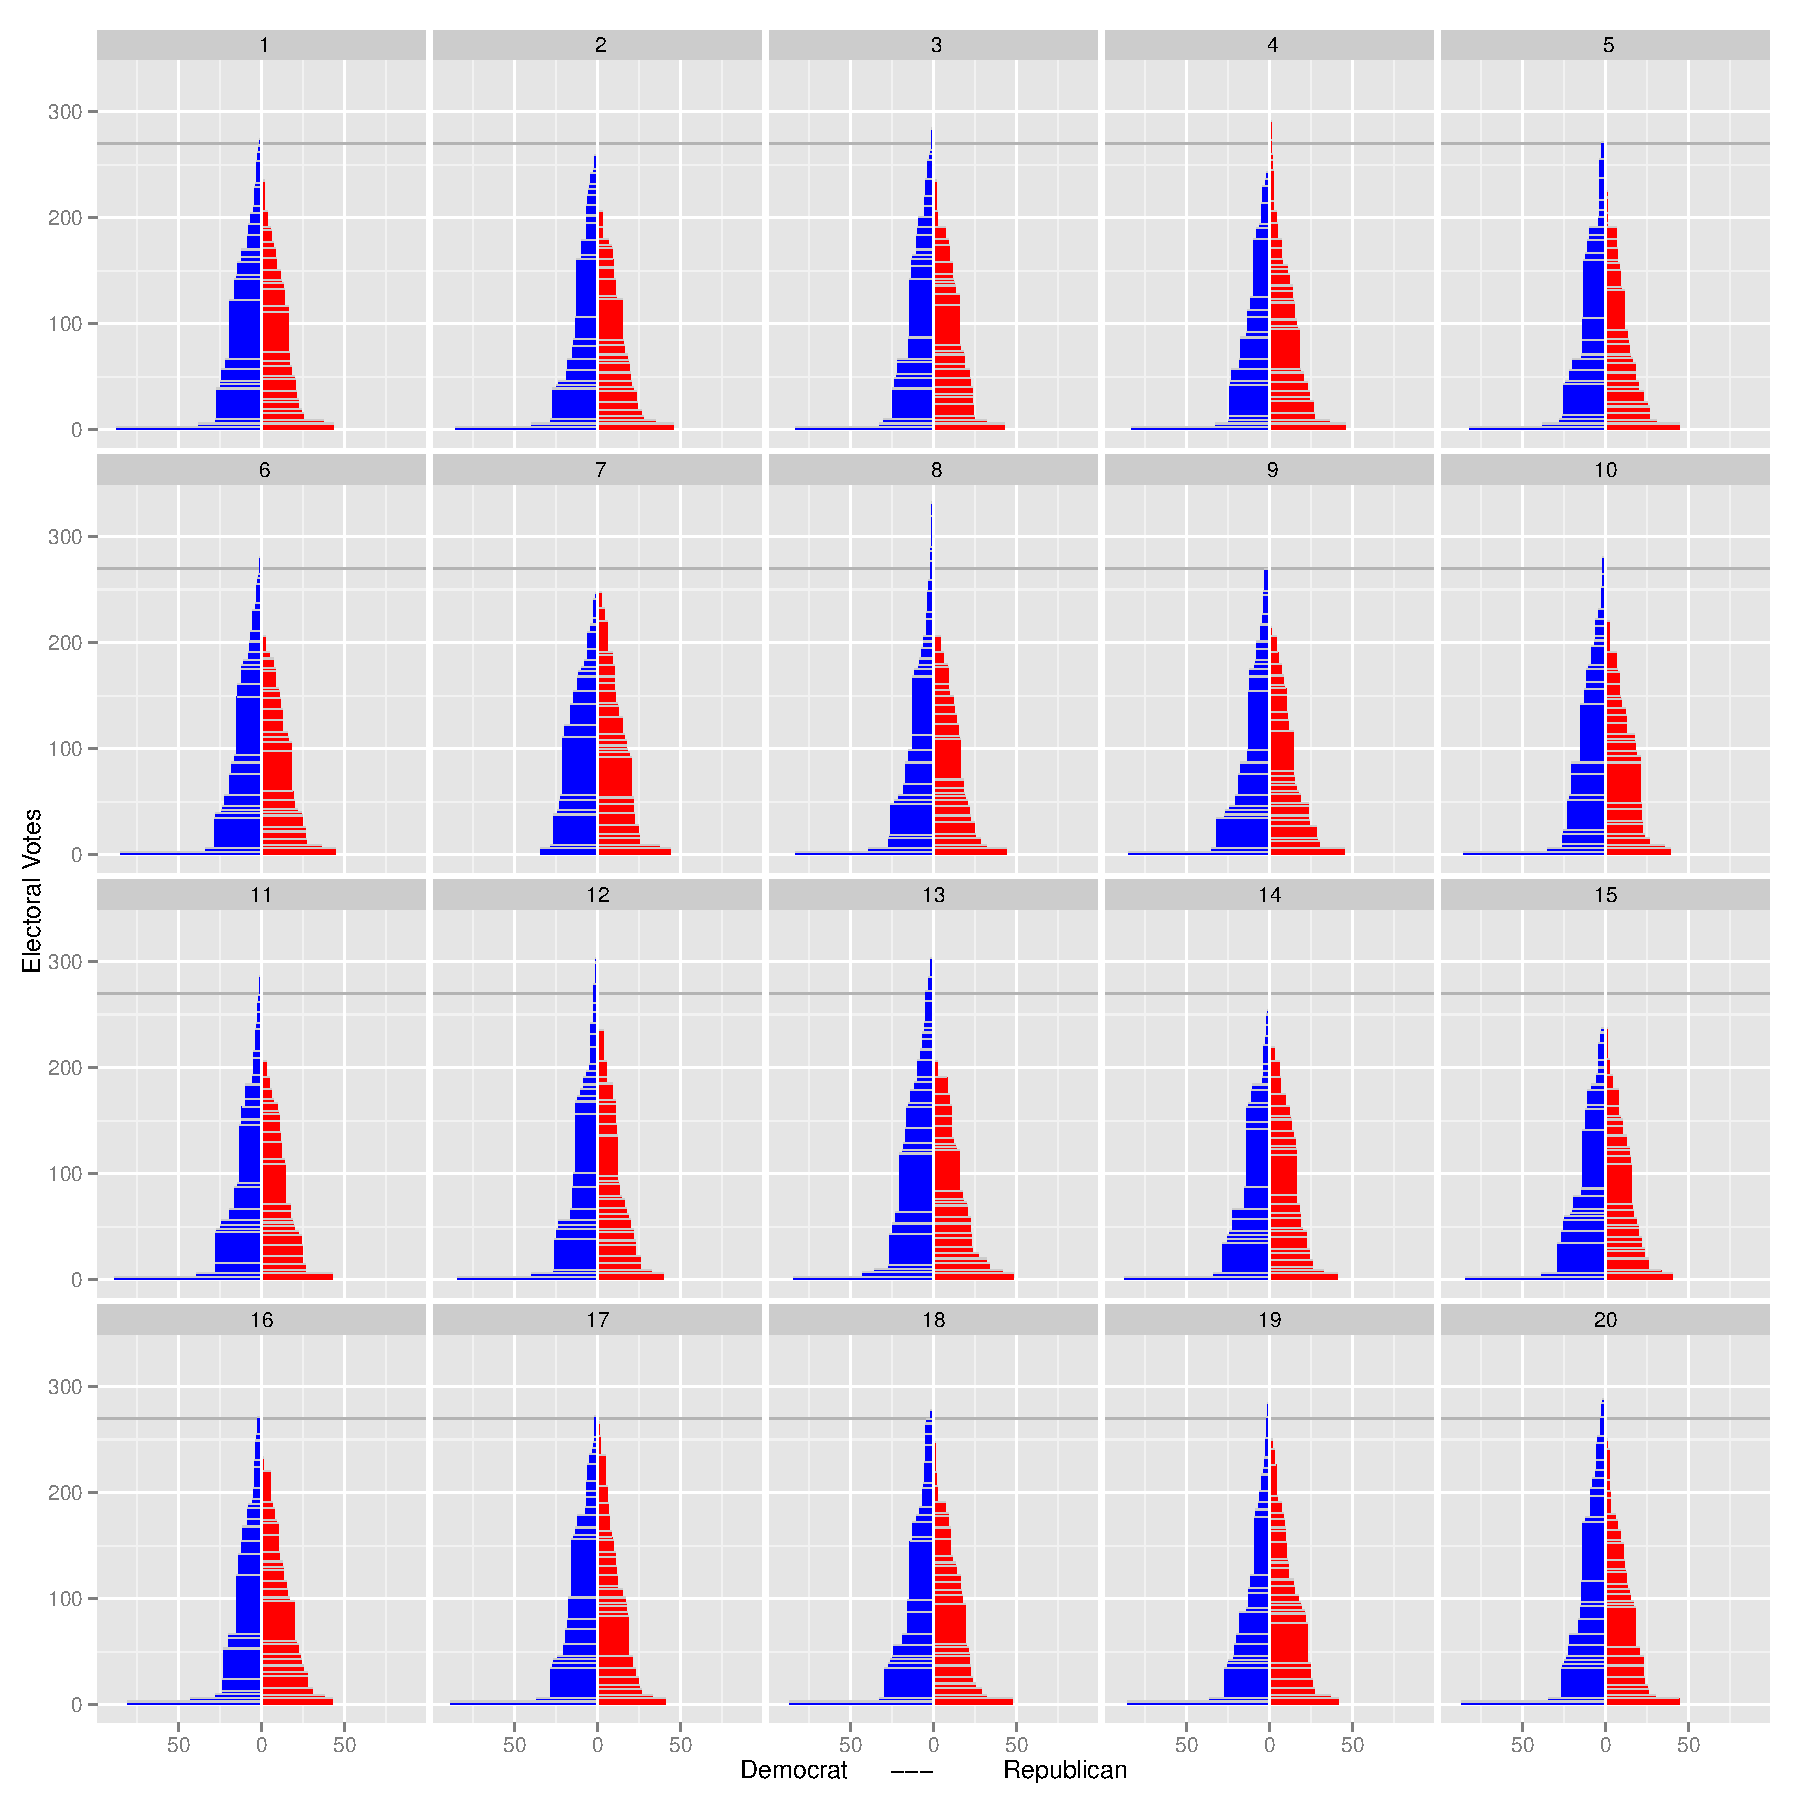
\includegraphics[width=0.99\textwidth]{tower.pdf} 
   \caption{ \label{fig:tower} Which of these towers is the most extreme? Which side is higher?}
\end{figure}

%The rest of the 19 plots are generated from the assumption that there is no difference between two groups of data. For this, the group structure of the data is broken by random permutation of the groups. 

If the null hypothesis is true, the observed data should look similar to the rest of the plots in the lineup making it difficult to detect the observed plot. On the other hand, if the null hypothesis is not true, the observed data should be different from the rest of the plots in the lineup and observers should be able to pick the data plot out from the rest.


A lineup can be evaluated by a single person or multiple observers. Based on the observer feedback the $p$-value is computed \citep{majumder:2013} and finally a decision is made about the hypothesis being tested.

%\begin{figure}[htbp] 
%   \centering
%   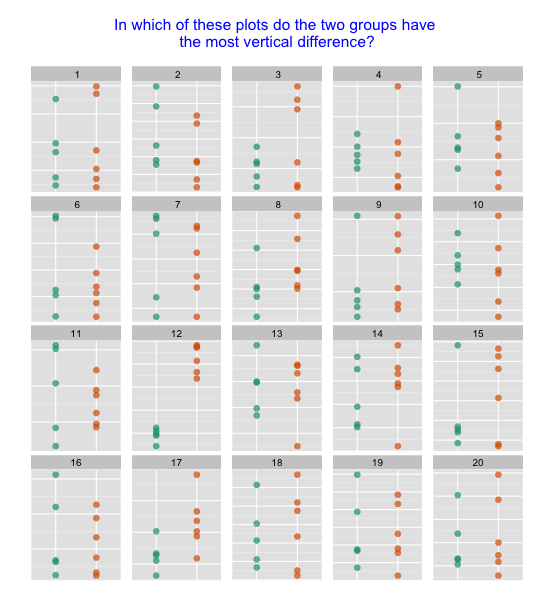
\includegraphics[width=6.5in]{plot_turk9_geno_4_3.png} 
%   \caption{A lineup of 20 plots. One of the plots is observed data and rest of the 19 plots are obtained by randomly permuting the group structure. Can you identify the observed data?}
%   \label{fig:lineup_geno}
%\end{figure}



\subsection{Observer task} Observer who evaluates a lineup do not necessarily be aware of the data that constitue a lineup. In response to a specific question the observer is to make a choice based on what he or she sees in the lineup. The choice could be right or wrong depending on whether the data plot is selected or not. Under null hypothesis, all the null plots look similar to what the observed data plot appears to be. This would make it harder to detect the observed data plot in the lineup. It is not expected that an observer would be able to detect the data plot in this scenario. But since there are limited number of plots in a lineup which is 20 in this case, there is a 1/20 chance that the observer would pick the actual plot. This proportion is associated with the type-I error probability. On the other hand if null hypothesis is not true, the observed plot would be different than the null plots making it easier to be distinguished. When multiple observers evaluate a lineup, the proportion of correct response can be used to estimate the power of the visual test \citep{majumder:2013}. 

For a lineup with fixed difficulty, the proportion correct responses may vary for different observers. If an observer evaluates multiple lineups, the proportion of correct evaluations by the observer could be used as a measure of performance by an observer. The another way of measuring the performance of the observer could be the time taken by an observer to evaluate a lineup. Since performance would also depend on the lineup difficulty it is essential to adjust for lineup difficulty before estimating the performance of the observer.

Some of the factors that may affect the performance of the observer are discussed in Section \ref{sec:factor_performance}. In this paper we focus on estimating the learning effect of the observer in terms of both proportion correct and time taken to evaluate a lineup through the attempts made during the evaluation of multiple plots. We also estimate the location effect of the observed data plot in a lineup. The other factors are controlled in simulation experiments so that learning effect and location effect can be estimated.

This paper is organized as follows; Section \ref{sec:factor_performance} describes some of the factors that may affect the performance of the observer. Section \ref{sec:exp_design} describes the design of the simulation experiments and methods to estimate the learning trend of the observer and location effect of the actual plot in a lineup. Section \ref{sec:result_socio} presents the analysis of the experimental data and the results.

\subsection{Experiments pooled}


\begin{table*}[hbtp] 
\caption{Visual test statistics and question asked to the observers to answer while evaluating a lineup } 
\centering 
\begin{tabular}{m{0.5cm}m{2cm}m{3cm}m{7.5cm}} 
\hline\hline 
Case & Statistic & Test Statistic & Lineup question \\ [0.5ex] % inserts table %heading 
\hline 
1  & Box plot & \begin{minipage}[t]{3cm} 	\scalebox{0.45}{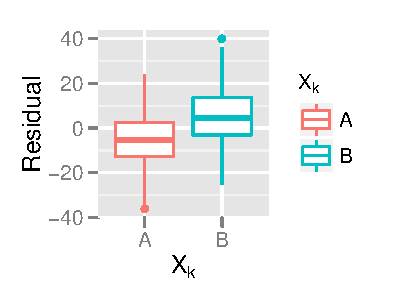
\includegraphics{stat_category.pdf}} \end{minipage} & Which set of box plots shows biggest vertical difference 
between group A and B? \\
2 &  Scatter plot & \begin{minipage}[t]{3cm}   \scalebox{0.45}{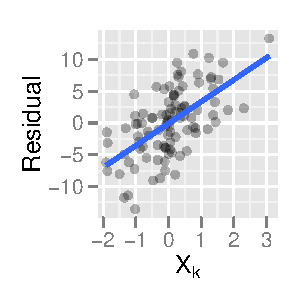
\includegraphics{stat_beta_k.pdf}}\end{minipage} & Of the scatter plots below which one shows data that has steepest slope? \\ 

\hline 
\end{tabular} 
\label{tbl:visual_stat} 
\end{table*} 


\section{Factors Affecting the performance of the observer} \label{sec:factor_performance} 

A brief description of the factors that may affect the power of visual inference.

\subsection{Signal in the data}

The visual test statistic is chosen so that it displays a specific patter in case the null hypothesis not true. Thus the most important factor that help an observer to correctly evaluate a lineup is the presence of any detectable signal in the data. On the other hand, if the null hypothesis is not true, visual test statistic should not display any distinguishable pattern. In fact, some of the null plots may appear to be the most different plot in a lineup influencing the observer to chose a plot different than actual data plot. This is an elegant feature of the lineup. It force the observer to chose a wrong plot when the null hypothesis should not be rejected.


\subsection{Choice of Visual Test Statistic}  The visual test statistic should be highly associated with the hypothesis under investigation. To achieve this purposes it is very important to decide which plot type and plot features should be adopted.  In a linear regression setting, the visual test statistics are presented in \citep{majumder:2013} for some common hypothesis testing.  It is also observed that a scatterplot may do a better job than a box plot when using as a visual test statistic for regression parameters.  Some of the effective features of visual test statistics are discussed in \citep{heike:2012} including plot type, color and shape of the plots.  \cite{niladri:2012} presents some \textit{distance measure} to determine how a plot may be different from each other.

Plots to do: for the same signal strength show the proportion correct for scatterplot and boxplot. eg., qplot(effect, ump-visual power, color= plot-type)

\subsection{Question that Human Observer Answers} The researcher knows about the underlying hypothesis but the observer does not necessarily know the underlying details of the lineup. So, the researcher needs to ask a question observer is to answer while evaluating the lineup. This question should provide the observer a little clue so that the answer reflects the hypothesized patterns in the actual plot. For example Table \ref{tbl:visual_stat} shows the questions asked for the simulation experiments done by  \citet{majumder:2013}. Notice that for case 1 if the observer can identify the actual plot in the lineup that should indicate that the plot chosen has the most vertical difference between groups A and B which is exactly what the researchers intend to examine. Similarly for case 2, a correct evaluation would indicate that the slope is different than the slope that may show up just from randomness.

These questions are very crucial for the power of visual test. They help observer think in a controlled direction. Notice that there may be unnecessary patterns in the actual data plot which may not necessarily indicate the existence of the significant signal in the plot. These question help observer not to be misguided by those patterns. To review further on this \citet{majumder:2013} have also asked why the observers choose a specific plot. 



%\subsection{Observer Personality} 

%\subsection{Visual Perception of Human Eye} Different people observe the lineup in different ways.  With the help of eye-tracking equipment \citet{zhao:2012} track the observers' eyes to see how they go through the plots in a lineup to come to their answers. The result suggest that people have particular methods of reading lineups. Some people read lineups from left to write direction while some read from upward to downward. Some people start looking from the center of the lineup while others start from the top left corner. In the earlier phase of the exercise, the observer tend to scan the plots and then start comparing plots to make a final decision. Beside right-left or up-down directions observer show some diagonal movement too. 
%
%Given this pattern of human eye tracks, it may effect the performance of an observer depending on where the actual plot is placed in the lineup. If the actual plot is on the top left corner and the observer starts from that point it may be easier to detect the actual plot earlier in the exercise and the observer could get plenty of time to make comparison. Thus the position of the actual plot in a lineup may have some impact.

\subsection{Demographics of Observer}  Some of the demographics of the observer such as age, gender, education level and geographical location may have effect on how an observer would examine the lineup. This may produce some variability in the performance of the observer. For example, a high school student may not respond same as a well educated person while evaluating a lineup. Also, to meet the Institutional Regulatory Board (IRB) requirement is is necessary to exclude any subject less than 18 years of old to participate human subject experiment. Thus we intend to only focus on the performance of observer with age 18 years or older. But still there may be variation in different age groups. Recruiting subjects with a well variety of age groups may be necessary to have control over this variability. 

Education level has some relation with age. Younger observer may not have higher degree. Thus some of the variability in performance for different education level may be confounded with age. On the other hand, it could be possible to have undergrad degree with higher age. Specially for any geographical location where not many certain gender group have higher education, this may occur. Thus the effect of all these demographical factors may be confounded at certain level. 

\subsection{Learning Trend of the Observer} When an observer evaluates a lineup he or she may learn something from the experience. If the same observer is shown another lineup the learning from previous evaluation may help. The more evaluations an observer makes the more skillful the observer may become. This learning trend may or may not be significant overall but it could influence the performance of the observer in some way. This paper investigates the learning trend with multiple simulation experiments.

\subsection{Location of Actual Plot in the Lineup} The actual data plot is placed in a random spot in a lineup. While evaluating the lineup some people may start looking from some specific part of the lineup. With the help of eye-tracking equipment \citet{zhao:2012} track the observers' eyes to see how they go through the plots in a lineup to come to their answers. The results suggest that people have particular methods of reading lineups. Some people read lineups from left to write direction while some read from upward to downward. Some people start looking from the center of the lineup while others start from the top left corner. In the earlier phase of the exercise, the observer tend to scan the plots and then start comparing plots to make a final decision. Beside right-left or up-down directions observer show some diagonal movement too. 

Given a specific pattern of eye movement of the observer in examining the lineup, the location of actual plot in the lineup may have some effect. Those who start exploring from the left top corner may get first glance of the actual plot if it is on that location. This should give the observer more time to compare it with the rest of the null plots. Those who start looking from the center may then scan towards right or left direction and thus don't have the chance to scan the null plots continuously as they could if they would start from a corner. Thus they should scan the center plot over and over again while scanning the left or right side plots. If the data plot is in the center location it may have multiple chance to be examined and hence be identified. 

It may be possible that some part of the lineup is little explored or not scanned by the observer if he or she feels that the actual plot is found before even seriously scanning the whole lineup. In those scenarios the location where the observer first start scanning is important. Placing the actual data plot in that location may yield different results.

\subsection{Selection of Null Plots} A lineup becomes difficult to evaluate if one of the null plots appears to be very similar to the actual plot. When null hypothesis is true it is a common scenario. With alternative hypothesis being true,  it may happen if  we compare actual plot with many null plots. But we have only specific number of null plots in a lineup. So, a different set of null plots may yield some variation in the difficulty of the lineup with the same actual plot. This may affect the performance of the observer while evaluating a lineup.

\subsection{Individual Performance of the Observer} Each person is different from others in some way. For example, in a controlled experimental study \citet{zhao:2012}  notice that some people spend a lot of time to decide no matter whether the lineup is difficult or easy while some simply glance at lineups to make a decision. This influences the response of the observer. Also subject specific variation in the power of visual test is observed in \citep{majumder:2013}. 

\section{Simulation Experiment and Methods}\label{sec:exp_design}
The performance of the observer while evaluating a lineup would depend on the factors described in Section \ref{sec:factor_performance}. In this section we present the experimental design to control some  of them so that learning effect of observer and location effect of a plot in the lineup can be estimated.

\subsection{Experiment Setup}  Multiple simulation experiments are designed to investigate the learning trend of the observer and the location effect of the actual data in the lineup. These are explained in tis section.

\paragraph{Design for Learning Trend:} Learning trend of an observer can be observed in terms of performance over successive feedback when multiple lineups are shown for evaluation. Each subject is shown a total of 10 lineups. The lineups are not necessarily with the same difficulty levels. But the order of lineups is randomized. The responses of the lineups are recorded by attempt 1 through 10. Attempt 1 means the response is for the first lineup and attempt 10 means the response is for the 10th lineup. The goal is to estimate whether performance of the observer improves from attempt 1 to attempt 10.

\paragraph{Design for Location effect:} The experiment is set up based on the gene expression data with two groups. The groups are defined based on the presence or absence of iron sufficiency. The null hypothesis is that there is no difference between this two groups. Null plots are obtained by randomizing the group structure of the data. The actual plot is then randomly placed in five different locations. For each location, five different sets of null plots are used to produce five different lineups. This produces 25 different lineups. One such lineup is shown in Figure \ref{fig:lineup_geno}. Similar procedure is applied to obtain 25 lineups to test the interaction between Genotype and Empty Vector (EV).

Each observer is shown three lineups. First lineups shown is a randomly selected Interaction lineup, then one from randomly selected Genotype lineup. Finally a test lineup is shown to screen out unusual evaluation. The subject is not aware which one is the test plot but it is informed in the starting of the task about having a test plot. The test plot is very easy and everyone should detect the data plot. The MTurk worker is paid based on whether he or she could correctly detect the data plot. But the data on test plot are excluded from the analysis.

\subsection{Data collection methods}  The human observers who evaluate the experimental lineups are recruited through Amazon Mechanical Turk \cite{turk} or MTurk Web site.  It is an online work place where people from around the world can perform some tasks and get paid. Usually tasks are very simple and no specialized training is required. Being a human is the main requirement. Tasks are designed for anyone to do but some tasks may require that workers satisfy some skill level depending on the recruiters need. The tasks are designed such that it does not take much time to complete. Humans are still better than computers in performing these types of tasks. The the amount of money paid for each task is very small as well. 

It is very fast, cheap and reliable to recruit people from MTurk. Thats why it is getting very popular among the researchers who perform human subject experiment. The another benefit is that a very diverse pool of subjects can be recruited which is otherwise very hard to obtain for a study. The researchers can easily filter the workers based on their experimental design, such as recruiting people only from a specific geographical location or a group of people who satisfy certain criteria etc. The recruiter can decide who they pay or not. Workers have to satisfy the task requirement to ensure payment. But at the end it is the recruiter who has the final say. Usually recruiters pay promptly after the task has been done properly and thats why MTurk is very popular among the online job seeker. At any point of time thousands of tasks are available for the thousands of workers around the world. 

Because of its convenience it is getting popular for scientific research study. In comparison with a lab study \cite{suri:2010} perform the same study using MTurk and demonstrate that their study results are as good as the lab study results even though MTurk study required less time and cost while provided more convenience. \cite{majumder:2013} recruited people from MTurk for their simulation study in estimating the power of visual statistical inference. They have done numerous pilot studies in lab before doing actual MTurk study and found similar results. \cite{mason:2012} explains various features of MTurk and describes how it can be used as part of human behavioral study.

We design and develop a web site which enables to display the lineups to the observers as per experimental design. The MTurk workers are redirect to the web site and the data are collected and automatically stored into a local server. Demographic informations such as age group, gender and education levels were collected. The time taken for each evaluation is computed based on the time the plot was shown and the time the feedback is received. The location of the observer is determined by the ip address of the observer.

\subsection{Model to Estimate Learning Trend}

The feedback provided by each observer on a lineup is a binary response variable. Suppose $Y_{ijk}$ denotes the response from observer $i$ on a  lineup $j$ in his/her $k$th attempt.  $Y_{ijk}=1$ if the response is correct otherwise  $Y_{ijk}=0$. 

%As per the design of the experiment for learning trend we have two different response variables. One is observer feedback on a lineup which is a binary variable.  The other variable is the time taken for each evaluation which is a continuous variable. Suppose random variable $Y_{\ell, i}$ denotes the response from subject $ i=1,2, ..., I$ on lineup $\ell=1,2, ..., L$. We model the mean $\mu_{\ell, i} = E(Y_{\ell, i})$ with a generalized liner mixed effect model
%
%\begin{equation} \label{eqn:trend}
%g( \mu_{\ell, i} )= W_{\ell i} \delta +  Z_{\ell i}  \tau_{\ell i},  
%\end{equation}

%\hh{
Let $\pi_{ijk}=  E(Y_{ijk})$ be the probability that  observer $i$ correctly picks the data panel from lineup $j$ in his/her $k$th attempt. We model this in a generalized mixed effects model of the form
\begin{equation} \label{eqn:trend_response}
g( \pi_{ijk} )= \mu + \alpha_k + u_i +  a_{i} k + \ell_j,  
\end{equation}
where $\mu$ is an overall average probability for picking out the data plot from a lineup, $\alpha_k$ is the effect of the $k$th attempt on the probability, with $\alpha_1 = 0$ and $k = 1, ..., K$.
$u_i$ and $a_i$ are observer specific random effects, $i = 1, ..., I$. $u_i$ is a random intercept, describing a basic subject-specific ability. We assume $u_i \sim N(0, \sigma_u^2)$. 
$a_i$ is a random slope capturing an individuals' specific learning effect over the course of $K$ attempts. We assume $a_i \sim N(0, \sigma_a^2)$. 
For $\ell_j$ we again assume a normal distribution, $N(0, \sigma_\ell^2)$. $\ell_j$ is a random intercept predicting lineup difficulty level. $g(.)$ denotes the {\it logit} link function $g(\pi)=g_1(\pi)=\log(\pi) - \log(1-\pi); 0 \le \pi \le 1$ . 

%$W$ is a design matrix of covariates corresponding to specifics of lineup $\ell$ and subject $i$, and $\delta$ is the vector of corresponding parameters. Covariates could include  demographic information of individuals, such as age, gender, education level etc.,  as well as the attempt made by the observer. $Z_{\ell i}$,  $1 \le i \le K$, $1 \le \ell \le L$,  is a design matrix corresponding to random effects specific to individual $i$ and lineup $\ell$; and 
%$\tau$  is a vector of independent normally distributed random variables $\tau_{\ell i}$ with  variance matrix $\sigma_\tau I_{KL \times KL}$. $\tau$ will usually include a component incorporating an individual's ability or skill to evaluate lineups. 

The inverse link function, $g^{-1}(.)$, from  Equation \ref{eqn:trend_response} leads to the estimate of the subject and the lineup specific probability of successful evaluation in $kth$ attempt by a single observer as 
\begin{equation} \label{eqn:trend_power}
\hat p_{ijk} =  g^{-1}(\hat{\mu} + \hat{\alpha}_k + \hat{u}_i +  \hat{a}_i k + \hat{\ell}_j).
\end{equation}

The learning of each observer over a course of $K$ evaluations may be observed as the improvement of the time taken to evaluate a lineup in the later attempts. Suppose $Z_{ijk}$ denotes the time taken for an observer $i$ to evaluate a  lineup $j$ in his/her $k$th attempt. Let $\mu_{ijk}=  E(Z_{ijk})$ be the average time taken by  observer $i$ to pick the data panel from lineup $j$ in his/her $k$th attempt. We model this in a generalized mixed effects model of the form
\hh{
\begin{equation} \label{eqn:trend_time}
g( \mu_{ijk} )= \mu + \alpha_1 + \alpha k + u_i +  a_{i} k + \ell_j,  
\end{equation}
where $g$ is now the inverse link function $g(\mu) = 1/\mu$ for positive values of $\mu$. $\mu$ represents the inverse of the overall average time taken by an observer to evaluate a lineup. $\alpha$ is the average change in time taken for each additional attempt.  $\alpha_1$ is an offset in time taken for the first effect. All other effects are random effects: as before, $u_i$ is a subject-specific intercept representing  individual speed of an observer with $u_i \sim N(0, \sigma_u^2)$. $a_i$ is a subject-specific slope representing the deviation of the speed-up (or -down) by attempt $k$. We assume $a_i \sim N(0, \sigma_a^2)$.
$\ell_j$ is a lineup-specific random effect for the time needed to evaluate a lineup; $\ell_j \sim N(0, \sigma_\ell^2)$.
}
\begin{equation} \label{eqn:trend_time}
g_1( \mu_{ijk} )= \mu_1 + \alpha_k + u_i +  a_{i} k + \ell_j,  
\end{equation}
where the link function $g_1(\mu)=1/\mu;  \mu >0$ and $\mu_1$ represents the inverse of overall average time taken to evaluate a lineup. 

The inverse link function, $g_1^{-1}(.)$, from  Equation \ref{eqn:trend_time} leads to the estimate of the subject and the lineup specific time taken for an evaluation in $kth$ attempt by a single observer as 
\begin{equation} \label{eqn:trend_power}
\hat \mu_{ijk} =  g_1^{-1}(\hat{\mu_1} + \hat{\alpha}_k + \hat{u}_i +  \hat{a}_i k + \hat{\ell}_j).
\end{equation}

%For $Y_{l,i}$ being binary response we use {\it logit} link function $g(\mu)=g_1(\mu)=\log(\mu) - \log(1-\mu); 0 \le \mu \le 1$ and $\hat p_{\ell i}$ gives the estimate of proportion correct by subject $i$ with lineup $\ell$.  The response time taken is a positive random variable with a right skewed distribution. For this the usual convention is to model a gamma distribution with time. Thus we used inverse link function $g(\mu)=g_2(\mu)=1/\mu;  \mu >0$ for gamma response $Y_{l,i}$ and $\hat p_{\ell i}$ gives the estimate of mean time taken by subject $i$ for lineup $\ell$.



\subsection{Model to Estimate Location Effect}


Since the actual data plot is same for each of the null sets of plot, the response data constitutes a multivariate response. Thus, to examine if the difference in proportion correct among the locations is statistically significant we fit a one way multi variate analysis of variance (MANOVA) model to the data.

Suppose $Y=(Y_1,Y_2, ... , Y_p)$ is a vector of random variable with dimension $p=5$ representing the response for five null sets. let $Y_{ij}$ represents $jth$ vector response for $ith$ location with $i=1,2, ..., 5$. We fit the following MANOVA model 
\begin{equation}\label{manova}
Y_{ij} = \mu_{i} + \epsilon_{ij}
\end{equation}
where $\mu_{i}= (\mu_{1i},\mu_{2i}, ..., \mu_{pi})$ is the mean vector for location $i$ and $Var(\epsilon_{ij})=\Sigma$. 


\section{Results}\label{sec:result_socio}

\subsection{Overview of the Data} Figure \ref{fig:turker_location} shows the location from where we received data. Notice that we received data from around the world and we observed diversity of location in the collected data. We notice diversity in not only location of the observers but also their gender, age groups and education levels. Table \ref{tbl:demographics} shows that number of male and female participants are almost same.

\begin{table}[hbtp]
\caption{Demographic information of the subjects participated the MTurk experiments. Average time taken for evaluating a lineup is shown in seconds.}
\centering
\begin{tabular}{rlrrr}
  \hline
 Factor & levels & subsjects & avg\_time & response \\ 
  \hline
Gender & Male & 1348 & 48.51 & 13493 \\ 
   & Female & 991 & 43.75 & 10564 \\ 
\hline
  Education & High school or less & 193 & 37.21 & 2241 \\ 
   & Some under graduate courses & 418 & 42.84 & 4070 \\ 
   & Under graduate degree & 584 & 44.29 & 5775 \\ 
   & Some graduate courses & 245 & 43.43 & 2460 \\ 
   & Graduate degree & 902 & 52.18 & 9511 \\ 
\hline
  Age & 18-25 & 740 & 42.97 & 7311 \\ 
   & 26-30 & 547 & 46.27 & 5585 \\ 
   & 31-35 & 376 & 44.27 & 3923 \\ 
   & 36-40 & 257 & 55.03 & 2714 \\ 
   & 41-45 & 141 & 43.90 & 1519 \\ 
   & 46-50 &  95 & 49.29 & 1003 \\ 
   & 51-55 &  83 & 48.67 & 867 \\ 
   & 56-60 &  64 & 59.73 & 678 \\ 
   & above 60 &  38 & 48.67 & 457 \\ 
\hline   
  Country  & United States & 1087 & 39.64 & 10769 \\  
  & India & 980 & 52.63 & 10227 \\ 
  & Rest of the world & 254 & 46.86 & 2819 \\ 
  
   \hline
\end{tabular}\label{tbl:demographics}
\end{table}


\begin{figure}[htbp] 
   \centering
   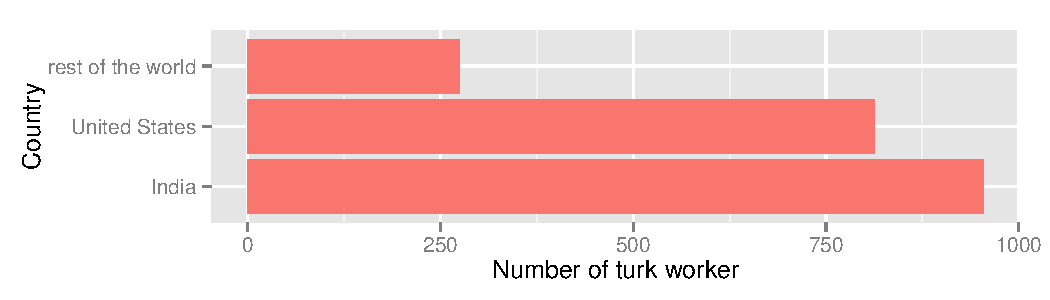
\includegraphics[width=4.5in]{turker_country.pdf} 
   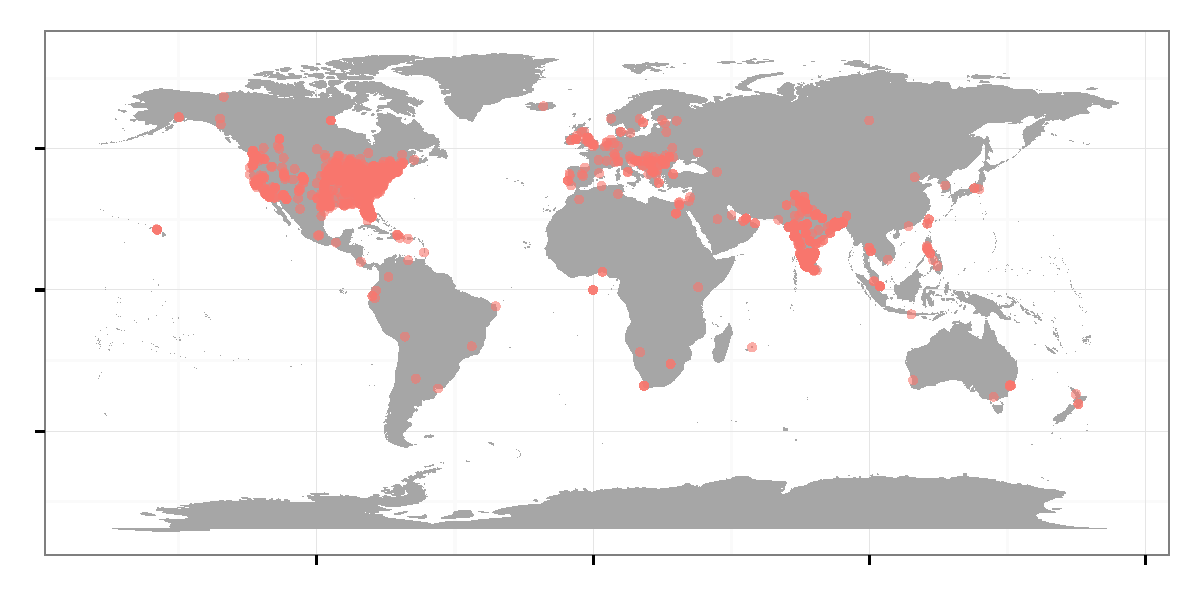
\includegraphics[width=4.5in]{turker_location.pdf}    
   \caption{Location of the Amazon Mechanical Turk workers participating our study. Most of the people are coming from India and United States even though there are people from around the world.}
   \label{fig:turker_location}
\end{figure}

The large number of participants are from age group 18 to 35. Interestingly we see many participants from older age groups as well. Specially for united states almost all the age groups show uniform participations after age 30 as in Figure \ref{fig:demographic_info}. Notice that fewer people participated from India beyond age 40 compared to united states. Even thoug total participations from india is larger compared to United States, they are mostly young people who are capable of using internet and computer. 


\subsection{Learning Trend} Each subject participating the experiment has seen multiple number of lineups for evaluations. Suppose $K$ be the number of lineups evaluated by a subject and $A_k$ be the $kth$ attempt, $k=1,2, ..., K$. Subjects may have a chance for self learning and do better on lineups shown later in the sequence. They may learn from their previous mistake or they may learn about the features of the plots being evaluated as they progress. Thus if there is any learning trend that should be apparent in proportion correct over $A_k$. But to obtain this we have to adjust for lineup difficulty and individual performances.

To accomplish this we fit generalized mixed effect model \eqref{eqn:trend_response} with lineups and subjects as random effect and no fixed effect. This gives the estimation of proportion correct responses  and we obtain residuals of the fitted model. The residuals give variations in proportion correct adjusted for lineup difficulties and individual skills. If there is any learning trend over different attempt $A_k$, the residuals should have that information since $A_k$ was not included as a covariate in the model. %At this point we focus on absolute residuals over different attempts to study the deviations due to attempts. An smaller absolute residual at attempt $A_k$ should indicate learning from all other attempts less than $k$. 

A plot of residuals against the attempts $A_k$ should reveal the trend if there is any. Figure \ref{fig:learning_trend} shows such plots for three experiments naming experiment 5, 6 and 7. For all the experiments we see some increasing trend of the residuals. This could be attributed to the exhaustion of subjects' attempt after some earlier evaluations are made.  But none of apparent trend are statistically significant. 


\begin{figure}[htbp] 
   \centering
   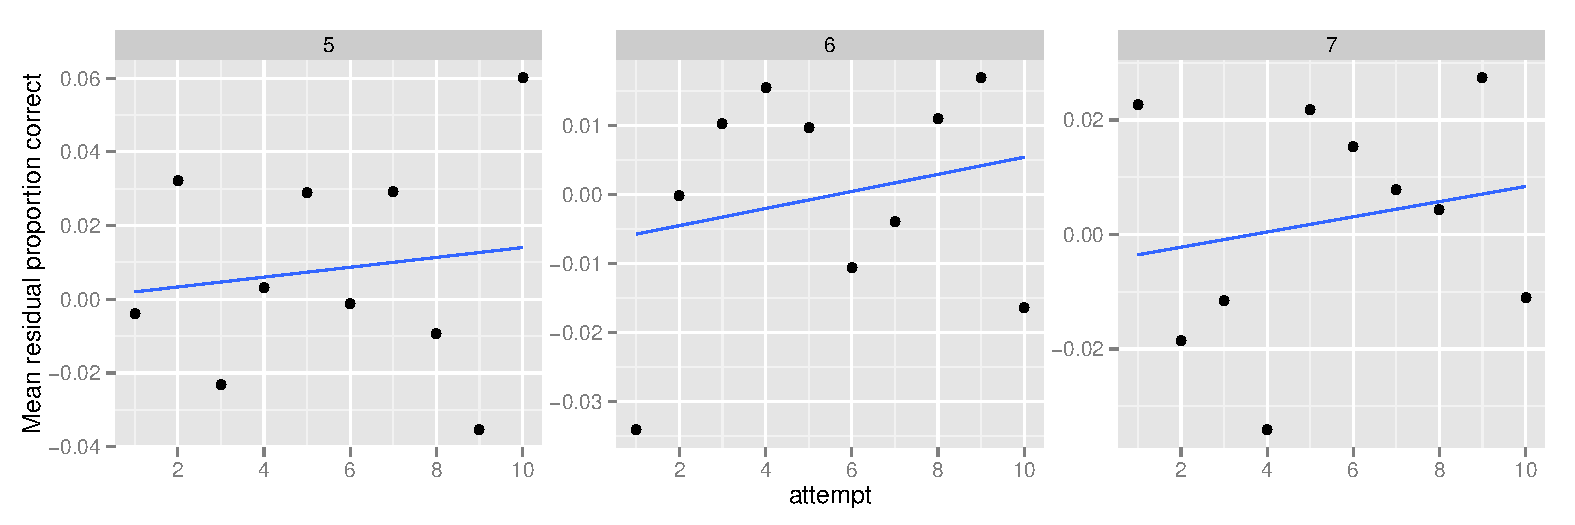
\includegraphics[width=6.5in]{learning_trend.pdf} 
   \caption{ Mean residuals of proportion correct obtained from the model \eqref{eqn:trend_response} fitted without attempt are plotted against attempt. A linear regression line through the points are shown. None of the slopes in these three experiments are statistically significant.}
   \label{fig:learning_trend}
\end{figure}

Learning trend is not only related to the proportion correct responses. It may be possible that people learn to answer fast. We examine this by the time taken for each evaluation. We fit a mixed effect linear model with time taken considering lineup and subjects as random effect. The resulting residuals are plotted in Figure \ref{fig:learning_trend_time}. It appears that in the later attempts observers take less time to evaluate a lineup. Even though it does not tell much about improving their performance over attempts, but it does indicate the improvement of their evaluation skill. Adding this information with what we observe in Figure \ref{fig:learning_trend}, we can say that the observers' improved skills could not contribute to their performance. It only help them finish the task faster in later attempts.

\begin{figure}[htbp] 
   \centering
   
\includegraphics[width=6.5in]{learning_trend_time.pdf} 
   \caption{Mean residuals of time taken obtained from model \eqref{eqn:trend_time} fitted without covariate attempt plotted against attempt. Linear regression lines are fitted through the points. For all the experiments the significantly downward slopes indicate that MTurk workers take less time as they progress through their attempts.}
   \label{fig:learning_trend_time}
\end{figure}


\subsection{Location Effect}

We set up a Turk experiment to examine whether there is any difference of performance based on the location of actual data plot in the lineup. For this five locations of a lineup were randomly chosen to put the same actual data plot. The locations are 2,9,12,16,20 for Interaction effect and 1,8,12,17,20 for Genotype effect. For a lineup with specific data plot location, five sets of null plots are used giving 5 lineups for each location. In total we have 25 lineups for Interaction effect and 25 lineups for Genotype effect. These 50 lineups are then evaluated by 100 people recruited from Amazon Mechanical Turk. Each person evaluated 3 lineups one from Interaction, one from Genotype and the third one was a test lineup. The test lineup is used to process the payment and examine the quality of the data and the responses of the test plot is not added to our analysis. 

The proportion of correct responses by the turk observers are shown in Figure \ref{fig:location_effect}. Notice that the data plot is same for each location but we see some variability of performance based on different null plots. This may happen if some null plots appear to be more similar to the actual plot while the others are not making some lineups harder than others even though the actual data plot is same. This pattern is evident in the Figure \ref{fig:location_effect} as we see proportion correct for null plot 5 is consistently above the null plot 1 for each of the locations. But this variability could be controlled at some extent by collecting more data for each location. Since the variability is larger when we have small number of responses as we see in the figure. For example, we have only one response for null plot 3 and 5 for Interaction effect which should lead to the extreme proportion of correct since one response would either be correct or wrong. 

\begin{figure}[htbp] 
   \centering
    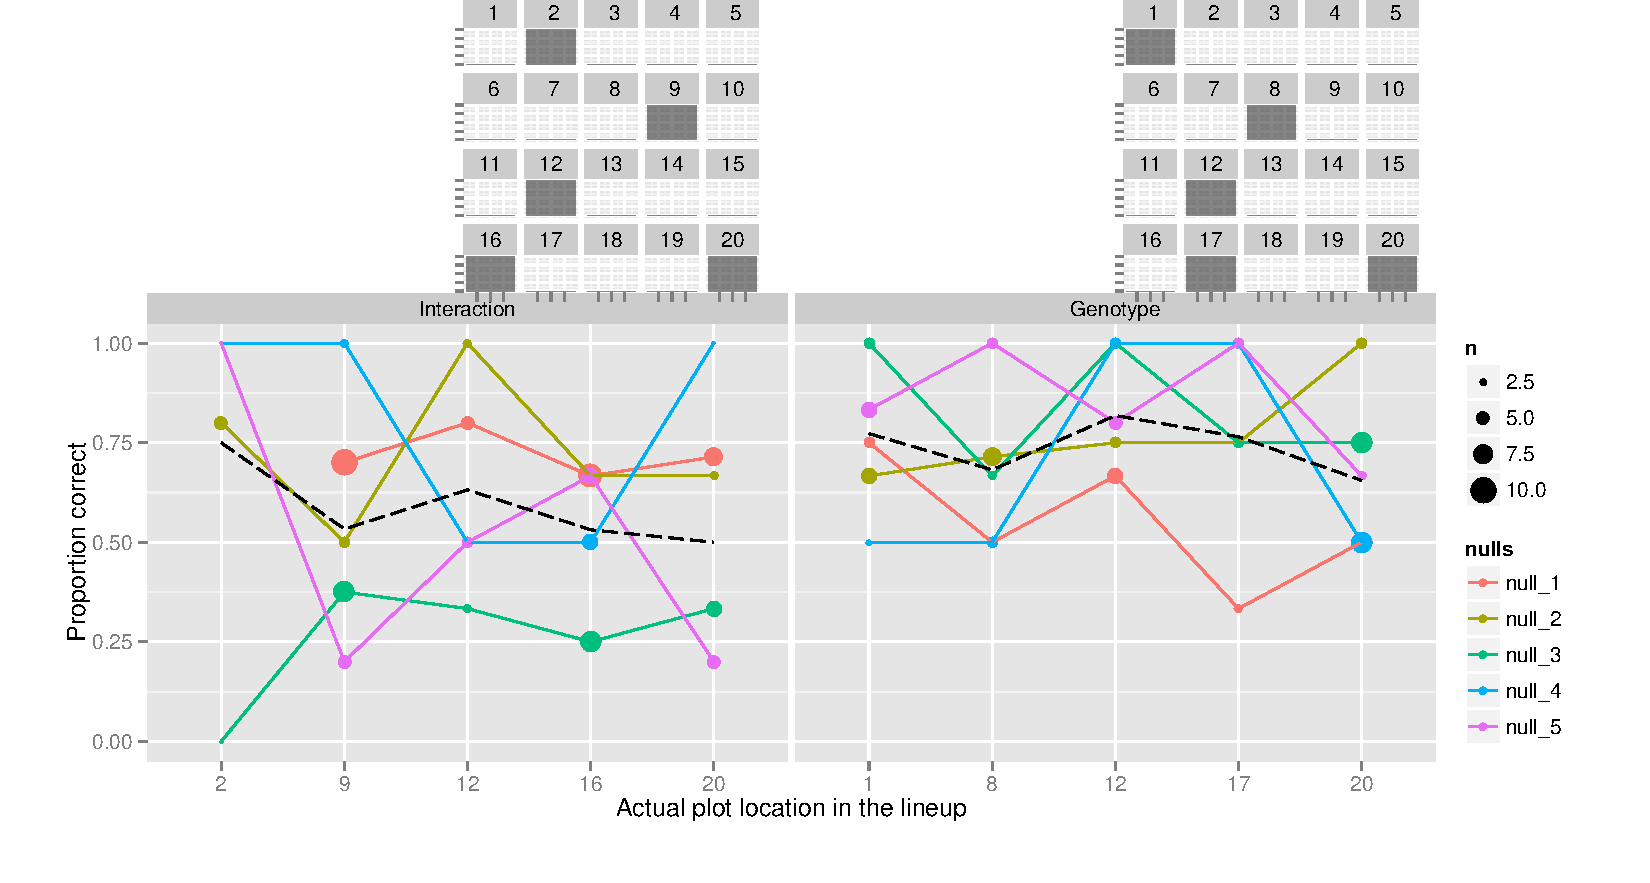
\includegraphics[width=6.5in]{proportion_nulls_guide.pdf} 
   \caption{Location of data plot in the lineup and proportion correct for both Interaction and Genotype effect. Each colored line represents a null set and the size of the dots represents number of responses. The overall average proportions are shown by dashed line. The actual data plot locations are shaded grey on the top panels to demonstrate their relative positions on a lineup.}
   \label{fig:location_effect}
\end{figure}

It is also interesting to check whether the proportion correct differs if the actual plot is on the outer boundary of the lineup or inside the outer boundary. As we see in Figure \ref{fig:location_effect}, location 9, 12 are inside for Interaction effect and location 8, 12 are inside for Genotype. It does not appear to have any difference whether the actual plot is inside or outer border of the lineup.

The overall proportion of correct response does not seem to vary much for different location indicating the non-existence of location effect. Model \eqref{manova} is used to test if the mean vectors are similar for different locations. To fit the model we use anova function of stats package of \cite{R:2012}. The results are shown in Table \ref{tbl:manova}. The $p$-values for both Interaction and Genotype effect are much bigger than the conventional threshold of 0.05 and we failed to reject the hypothesis that there is no difference in location. 

\begin{table}[hbtp]
\caption{The results obtained by fitting MANOVA Model \eqref{manova}.}
\begin{center}
\begin{tabular}{ccccccccc}
  \hline \hline
 Location & && & \multicolumn{3}{c} {Degrees of Freedom}  & F test \\
 \cline{5-7}
 Effect & DF & Pillai & Approx. F & Numerator& Denumerator &Residual & p value\\
  \hline
  Interaction& 3&1.4783 &0.7772&15&12 & 6 & 0.6821 \\ 
  Genotype &4&1.7796 &1.1221&20&28 & 8 &  0.3824 \\ 
   \hline
\end{tabular}
\end{center}
\label{tbl:manova}
\end{table}

We also fit Model \eqref{manova} with only two locations based on outer or inner plot location. By outer location we mean the data plot location which is on the border area of the lineup. For example inner locations of a lineup would be 7,8,9,12,13,14. It turns out that inner and outer locations are also not significantly different.





%% latex table generated in R 2.15.0 by xtable 1.7-0 package
%% Fri Sep  7 10:28:47 2012
%\begin{table}[hbtp]
%\caption{Fixed effect parameter estimates of generalized mixed model. Note that attempt is not significant for experiment 2. The continuous covariate, lineup difficulty, was measured by the $p$-value of the actual plot in the lineup.}
%\begin{center}
%\begin{tabular}{llrrrrl}
%  \hline
%& Parameters & Estimate & Std..Error & z.value & P-value  & \\ 
%  \hline
%\multicolumn{2}{l}{\bf{Experiment 1} } &&&& &\\
%&(Intercept) & -0.30 & 0.10 & -2.89 & 0.00 & ***\\ 
% & attempt & 0.08 & 0.02 & 4.21 & 0.00 & ***\\ 
% & lineup difficulty & -11.32 & 1.01 & -11.19 & 0.00 & ***\\ 
%\multicolumn{2}{l}{\bf{Experiment 2} } &&&&& \\
% & (Intercept) & 2.36 & 0.15 & 16.09 & 0.00 & ***\\ 
% & attempt & 0.01 & 0.03 & 0.35 & 0.72 \\ 
% & lineup difficulty & -55.03 & 2.20 & -25.00 & 0.00 & ***\\ 
%\multicolumn{2}{l}{\bf{Experiment 3} } &&&& \\
% & (Intercept) & 0.25 & 0.16 & 1.58 & 0.11 & .\\ 
% & attempt & 0.10 & 0.03 & 3.34 & 0.00 & ***\\ 
% & lineup difficulty & 3.00 & 0.56 & 5.36 & 0.00 & ***\\ 
%   \hline
%\end{tabular}
%\end{center}
%\label{tbl:model_par}
%\end{table}

% \footnote{Signif. codes: 0 �***� 0.001 �**� 0.01 �*� 0.05 �.� 0.1}


%------------------------------------------------------------------------------------
\paragraph{Acknowledgments}
%------------------------------------------------------------------------------------
This work was funded in part by National Science Foundation grant DMS 1007697. All studies were conducted with approval from the internal review board IRB 10-347.

\section{Conclusion}


With controlled simulation experiments, it is observed that the performance of human observers does not increase through successive attempts while evaluating multiple lineups. But their skill in evaluating the lineup in shorter time gets improved over successive evaluations. When an observer evaluates multiple lineups, the earlier evaluations take significantly longer than the later evaluations. This result is very important as it suggests that the power estimated for visual inference using human subject experiment is robust and may not change if those participants are allowed to give feedback again. This investigation suggest that the skilled person may only do it faster.

The simulation experiment reveals that the effect of location of actual data plot in the lineup is not significant. This is important as the visual statistical inference procedure suggests that the data plot be placed at random anywhere in the lineup. Even though there are variations on the performance depending on actual plot locations, it is not statistically significant to be of any concern. This paper suggests that any random place in a lineup is as good as other places in the lineup.

More experiments may be needed to make a concrete decision about the difference in power with skilled observer and a non-skilled observer in terms of statistical graphics. The numerous pilot studies done with the more trained participants suggest that power of visual statical inference may be higher with skilled observer. Thus the variations observed with individual performances could be attributed to individual abilities.  

This investigation allowed each observer to evaluate 10 lineups assuming that it would not cause fatigue or disinterest of the observers towards the experiment based on the pilot studies. The future research may involve doing more experiments to check if fewer or more than 10 lineups have any significant impact on performance of the observer. 

Also, a lineup with fewer or larger than 20 plots may yield different results. If the size of the lineup is much higher than 20, it is intuitive that there may be location effect of the data plot in the lineup. It is because, the observer may get tiered of scanning and make decision based on the partial scanning of the lineup. On the other hand fewer than 20 plots would give observer compare the actual plot with fewer null plots give more chance of picking actual plot as an error not as an actual plot. These are the some of the issues that needs to investigated.


\section{Some figures and tables (for review)}

\subsection{How people pick the data plot} In the experiment setup we have a question for the turk observers to choose the reason for their selection of a particular data plot. It is shown by \cite{majumder:2013} that these choice reasons reveal the way people picks the data plot in the lineup. To investigate this further we added free text input option for their choice reason instead of some fixed reasons to select from. In this experiment people could write whatever they think their reasons for choice are. Figure \ref{fig:wordle} shows the words used to explain their reasons for choice. The most common words used to explain their choice are points and green which indicates two important feature of a plot. One is the indicator of plot aesthetics and the other is the color. Spread, steepest, line and apart are some other important words used frequently. Spread and apart are indicative of variability in the data. Steepest and line indicates some sort of systematic pattern in the data.

\begin{figure}[htbp] 
   \centering
   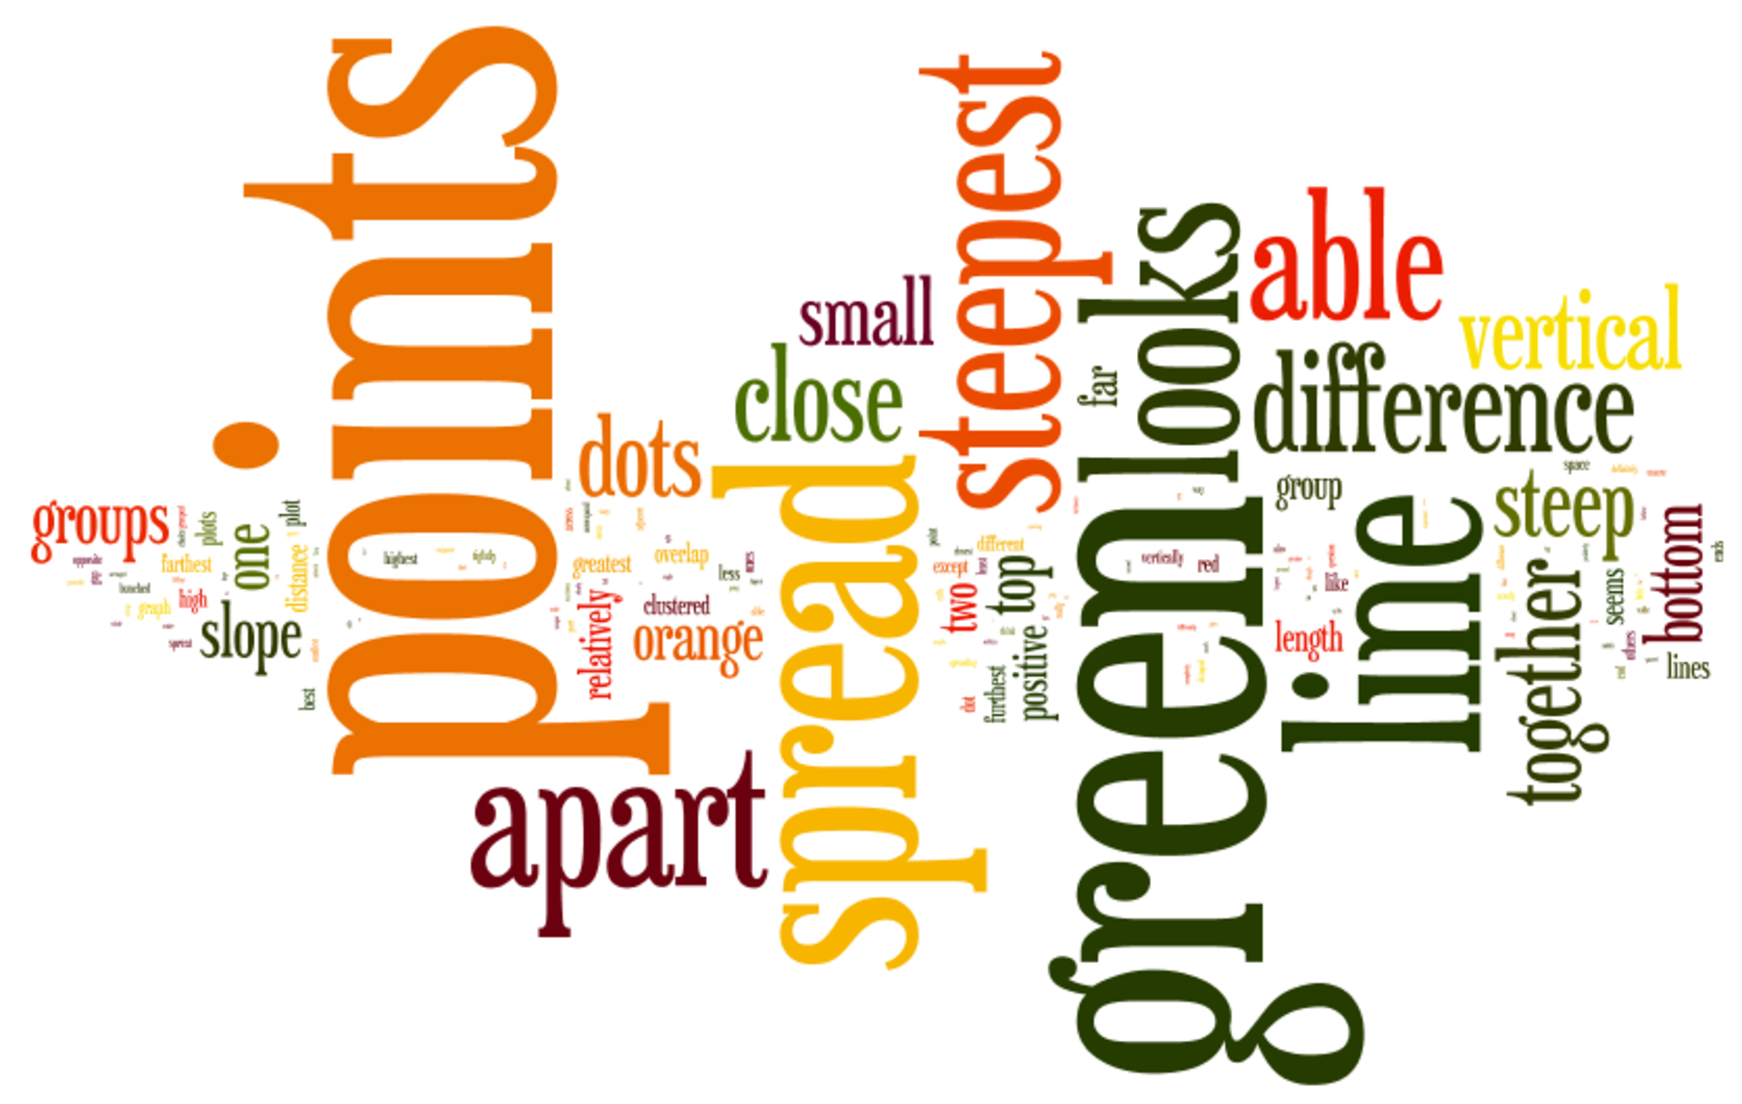
\includegraphics[width=3.5in]{reasoning_words.pdf} 
   \caption{Words used to explain the reasons for selection of data plot in a lineup show what features of a lineup may help a non-statistician to evaluate it. Larger font indicate more people choosing that word. Different color is used just to separate the words.}
   \label{fig:wordle}
\end{figure}

Figure \ref {fig:wordle} also shows some insight about peoples way of reading a plot. We notice that variability in the data, color and aesthetics used to generate plots and existence of any systematic pattern in the plot are some of the important features revealed from the figure. These features are commonly used by human brain to examine and compare plots. Notice that these features may be specific to this particular experiment. There could be different other features people would use to evaluate a lineup depending on the situation. But these words we have a general idea how people may think to evaluate a lineup.

Turk workers are not necessarily trained on statistics or aware of specific terms used in statistics or statistical plots. Thus it is also interesting to note that how they explain things that have specific definitions and meaning. Notice in Figure \ref {fig:wordle} that some keywords like spread, apart should be analogous to larger variability while together,  close may be for indicating smaller variability.


\begin{table}[hbtp]
\caption{Amazon mechanical turk experiments and their properties. Duration in hours per 100 tasks show the popularity of some tasks compared to others.}
\centering
\begin{tabular}{rlrrrrrrr}
  \hline
& Experiment& \multicolumn{2}{c}{ Total Task}& Average & \multicolumn{2}{c}{Duration (hour)} & Payment & Pay rate\\
\cline{3-4} \cline{6-7}
Serial & description & submitted & rejected & time(min) & Actual & 100 task& \$/task & \$/hour\\ 
  \hline
1 & Boxplot & 406 & 106 & 10.68 & 146.48 & 36.08 & 0.50 & 2.81 \\ 
  2 & Scatterplot & 359 &   9 & 10.80 & 42.68 & 11.89 & 1.00 & 5.58 \\ 
  3 & Contaminated plot & 219 &  19 & 13.53 & 126.17 & 57.61 & 1.00 & 2.22 \\ 
  4 & Polar vs Cartesian & 110 &  10 & 20.65 & 11.65 & 10.59 & 1.00 & 2.91 \\ 
  5 & Hist vs density & 234 &  37 & 17.85 & 41.57 & 17.76 & 1.00 & 3.36 \\ 
  6 & Violine vs boxplot & 417 &  17 & 17.95 & 105.87 & 25.39 & 1.00 & 3.34 \\ 
  7 & Group separation & 106 &   6 & 16.13 & 5.15 & 4.86 & 1.00 & 3.72 \\ 
  8 & Sine Illusion & 101 &   1 & 16.52 & 78.38 & 77.60 & 1.00 & 3.63 \\ 
  9 & Gene expression & 103 &   3 & 12.47 & 11.27 & 10.94 & 0.50 & 2.41 \\ 
  10 & Test normality & 406 &   6 & 22.70 & 74.35 & 18.31 & 1.00 & 2.64 \\ 
   \hline
\end{tabular}
\label{tbl:mturk}
\end{table}


\begin{figure}[htbp] 
   \centering
   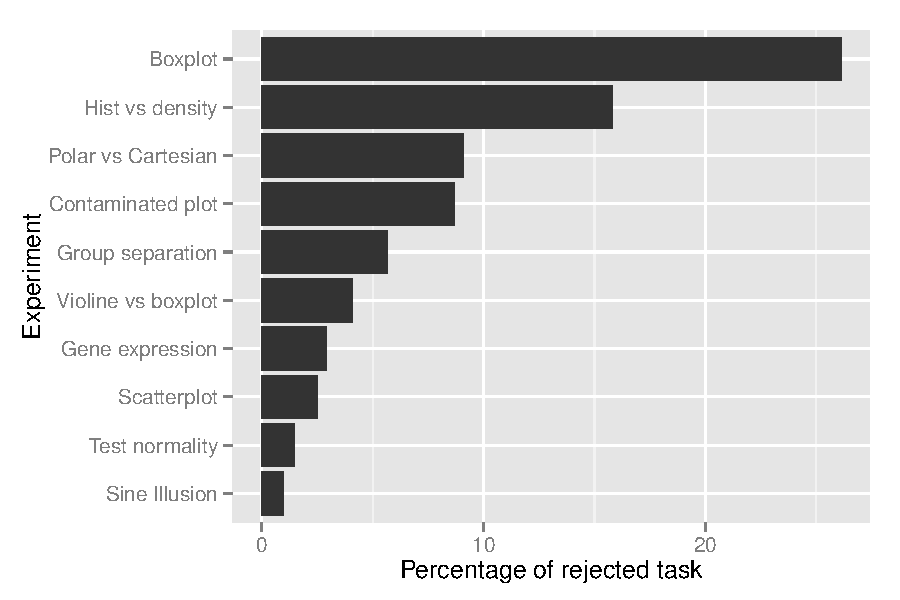
\includegraphics[width=3in]{rejected_task.pdf}
      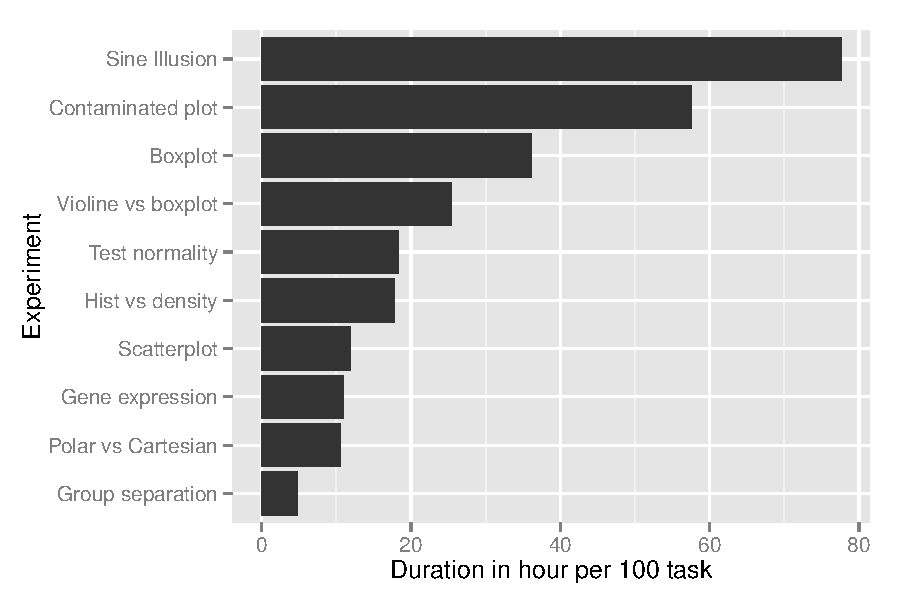
\includegraphics[width=3in]{task_duration.pdf} 
   \caption{Percentage of rejected tasks and duration of each experiment in hour per 100 tasks for each of the 10 experiments. Most of the tasks got rejected for box plot experiment.  Even though the sine illusion experiment took longest to finish the rejection rate is lowest for this experiment.}
   \label{fig:task_duration}
\end{figure}


\begin{figure}[htbp] 
   \centering
   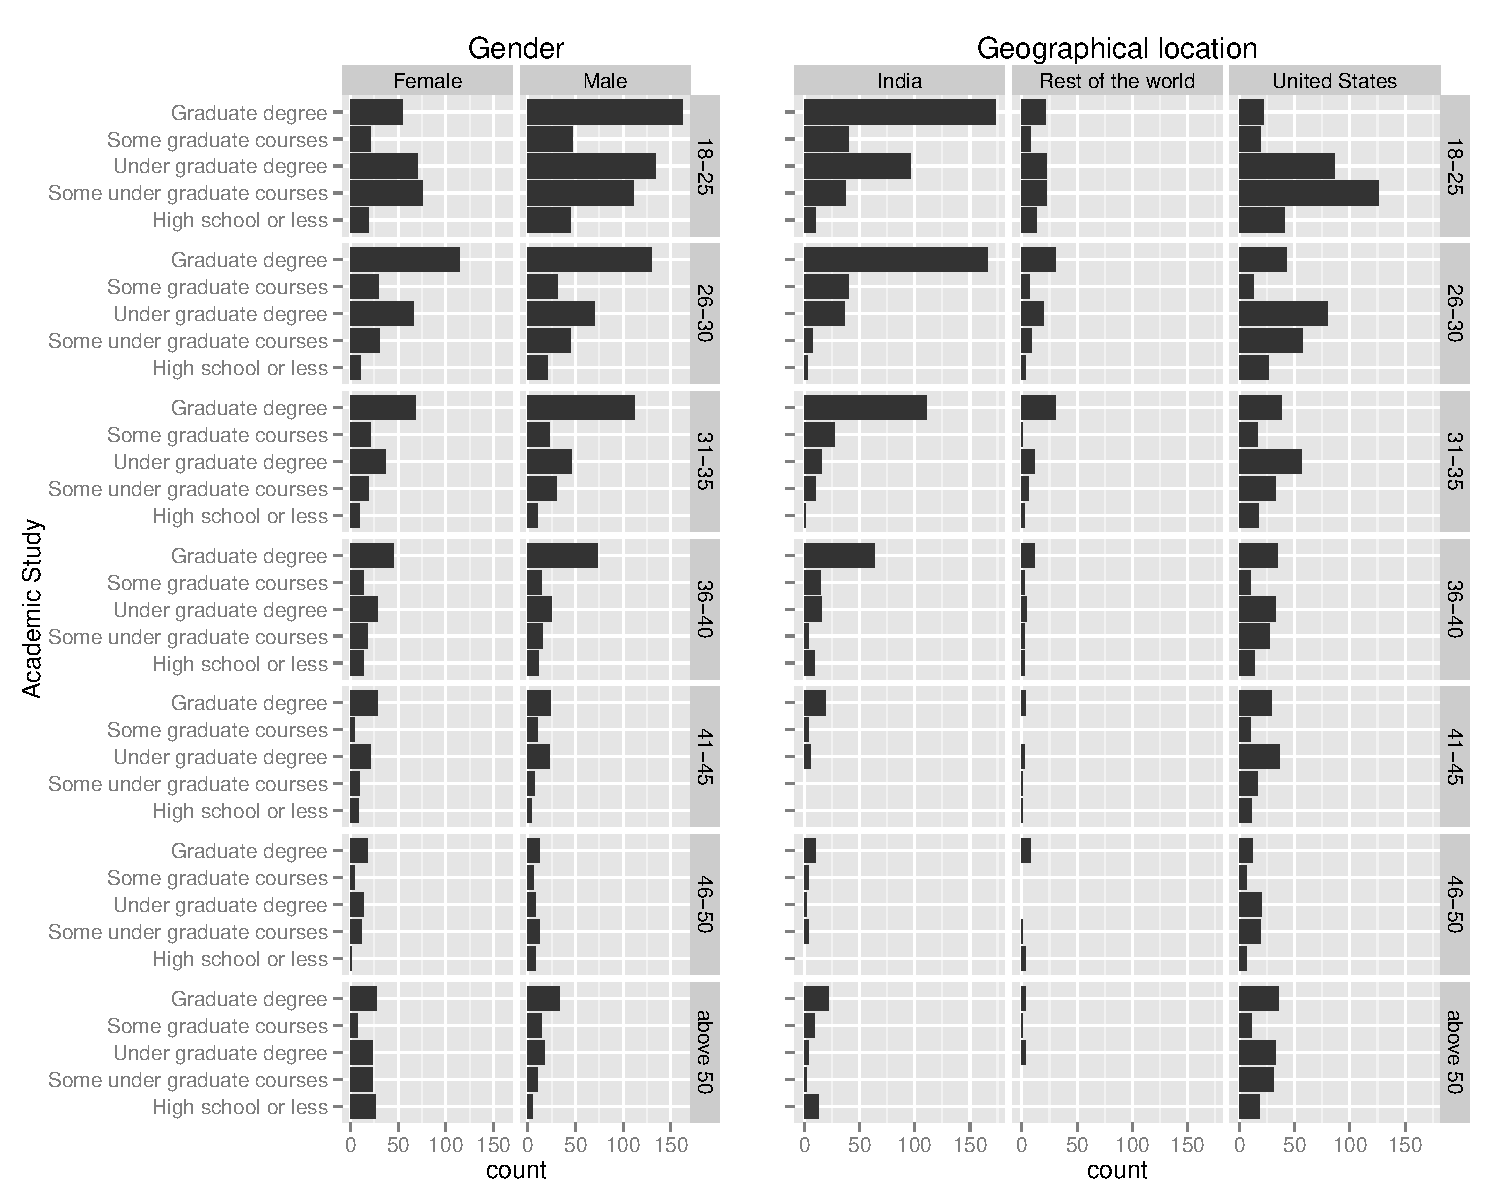
\includegraphics[width=6in]{demographic_info.pdf} 
   \caption{Countrywise distribution of age and academic levels of the MTurk workers participating the experiments shows the diversity of the subjects in all the demographic aspect. Almost equal number of male and female subjects participated the online experiments.}
   \label{fig:demographic_info}
\end{figure}


\begin{figure}[htbp] 
   \centering
   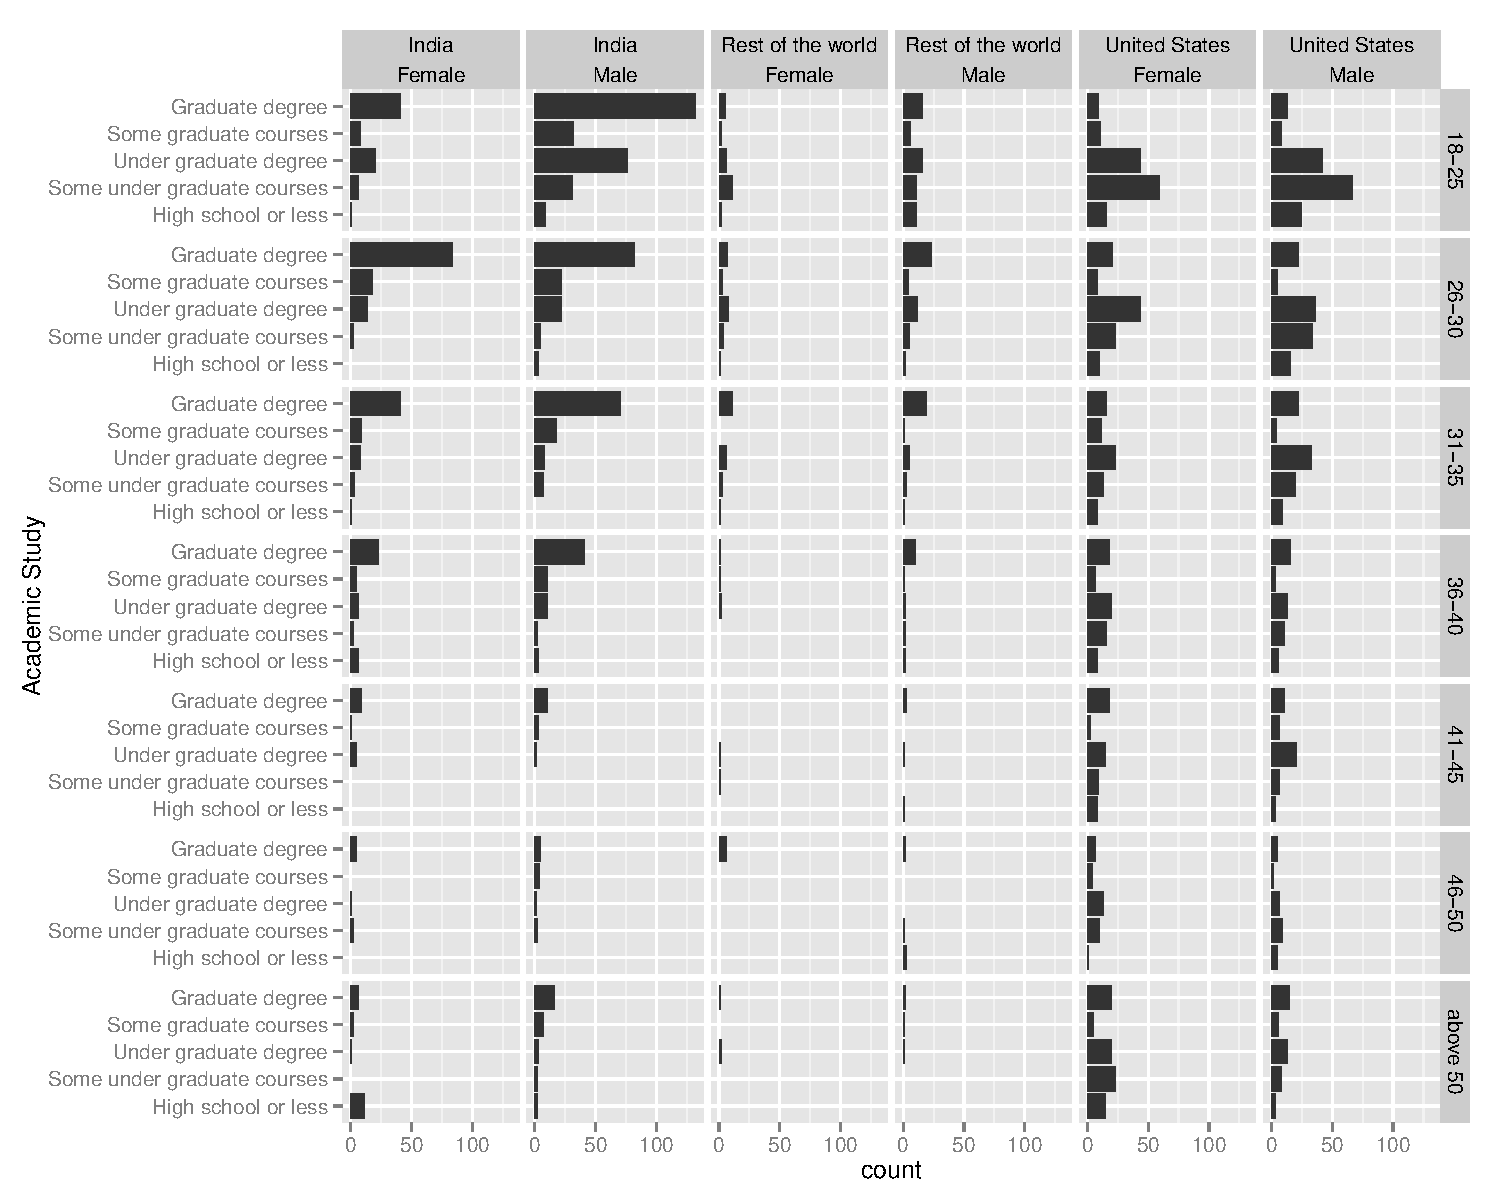
\includegraphics[width=6.5in]{age_gender_within_country_bar.pdf} 
   \caption{Countrywise distribution of age and academic levels of the MTurk workers participating the experiments shows the diversity of the subjects in all the demographic aspect. Male and female participants differ in India specially for agelevel 18-25. For United States number of participants are similar beyond age 40 while few number of participants coming from India beyond that age.}
   \label{fig:gender_country}
\end{figure}


\begin{figure}[htbp] 
   \centering
   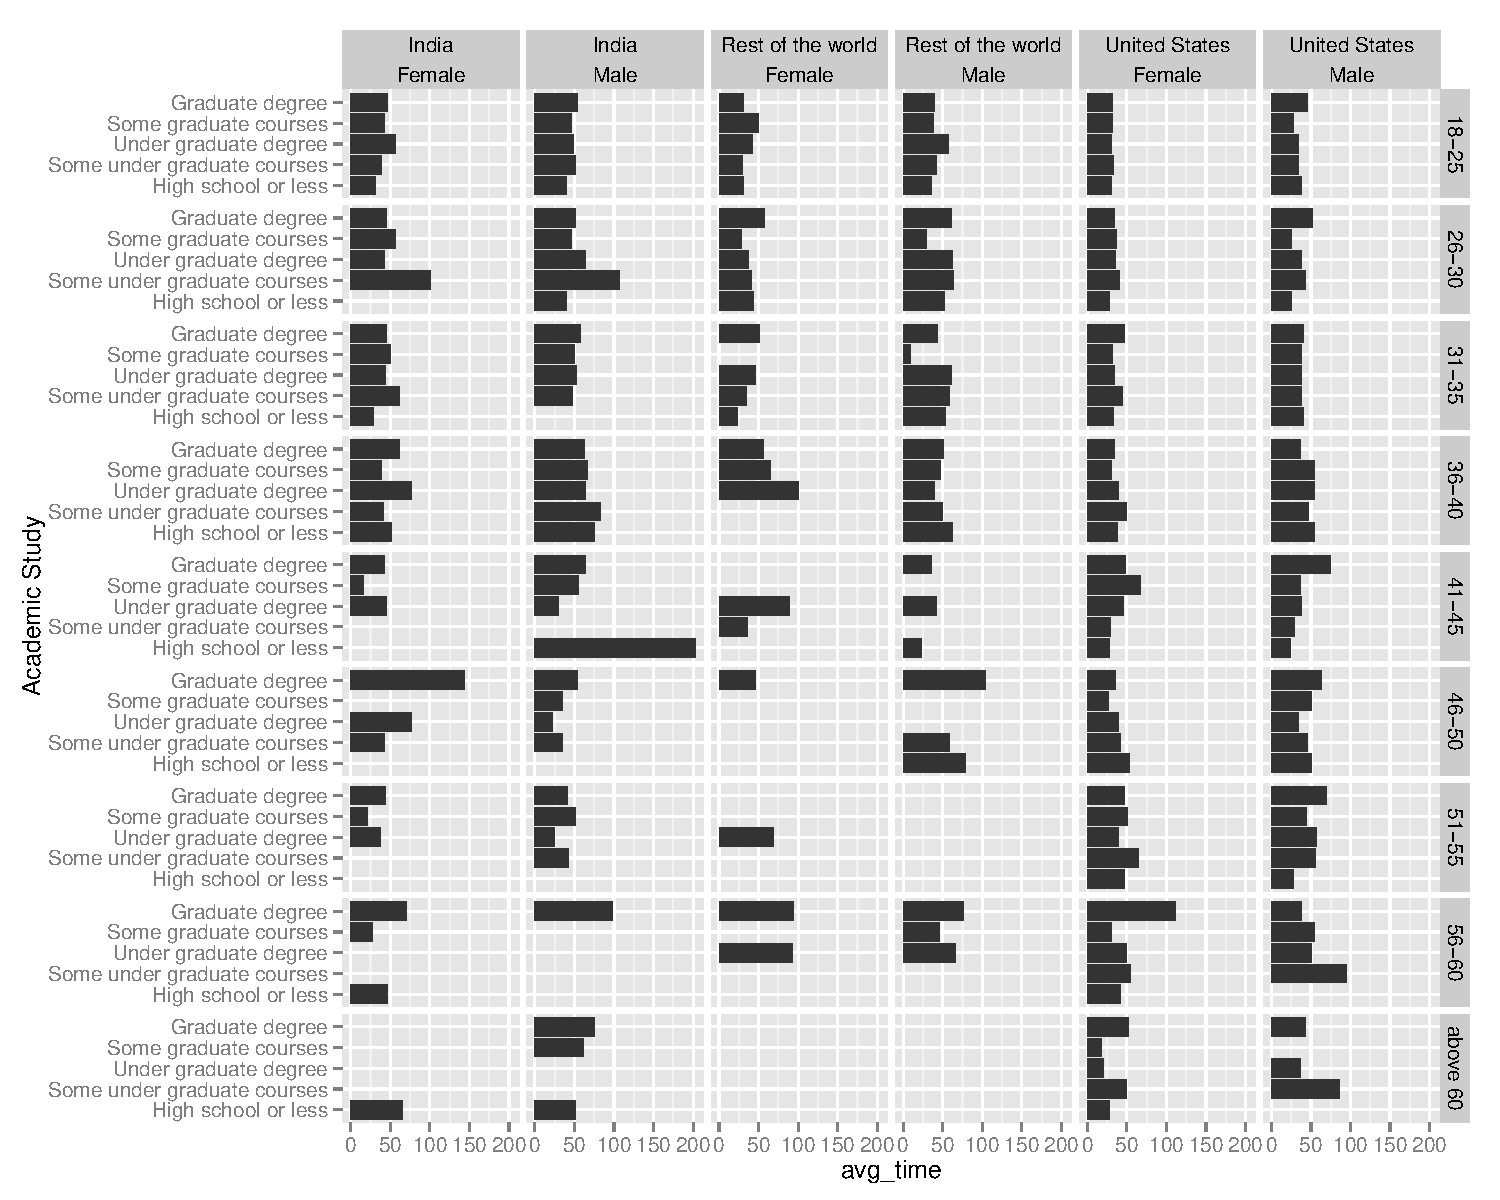
\includegraphics[width=6.5in]{age_gender_within_country_time.pdf} 
   \caption{Countrywise average time taken for different age and academic levels of the MTurk workers participating the experiments shows that the demographic factors may not have effect on time taken. }
   \label{fig:gender_country}
\end{figure}


\begin{figure}[htbp] 
   \centering
   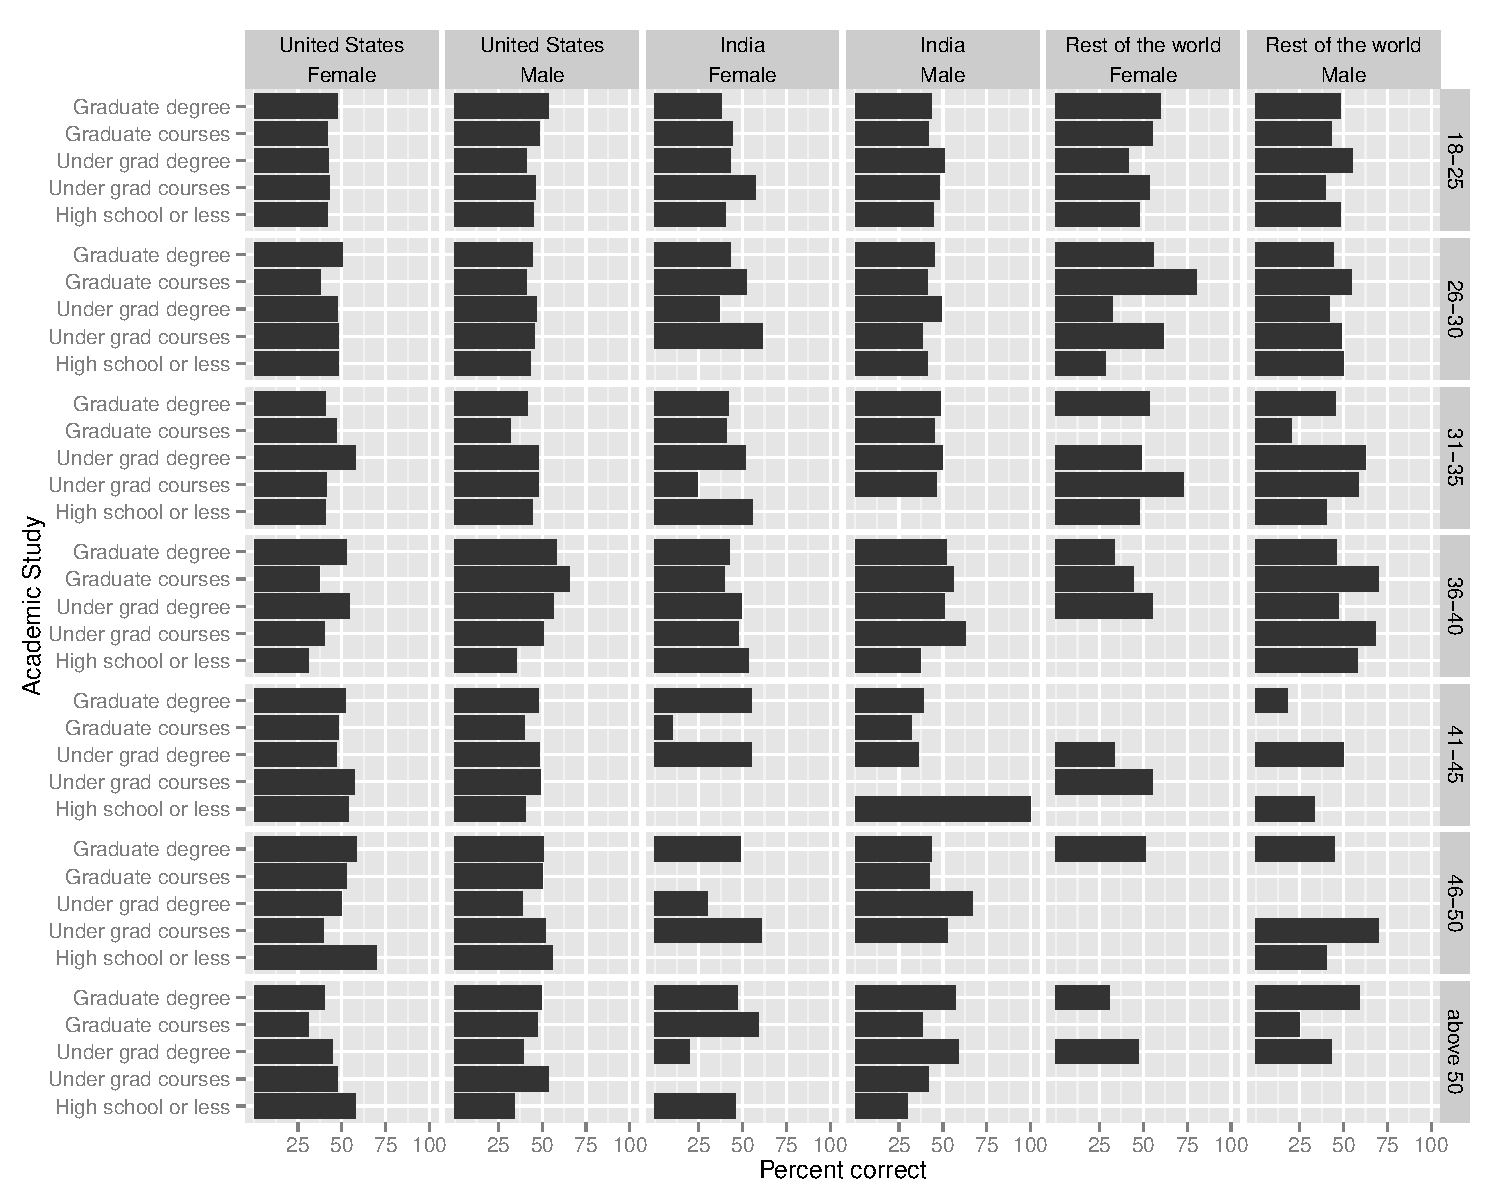
\includegraphics[width=6.5in]{age_gender_within_country_correct.pdf} 
   \caption{Countrywise percentage of correct responses for different age and academic levels of the MTurk workers participating the experiments shows that the demographic factors may not have effect on the percentage of correct responses. }
   \label{fig:gender_country}
\end{figure}


\begin{figure}[htbp] 
   \centering
   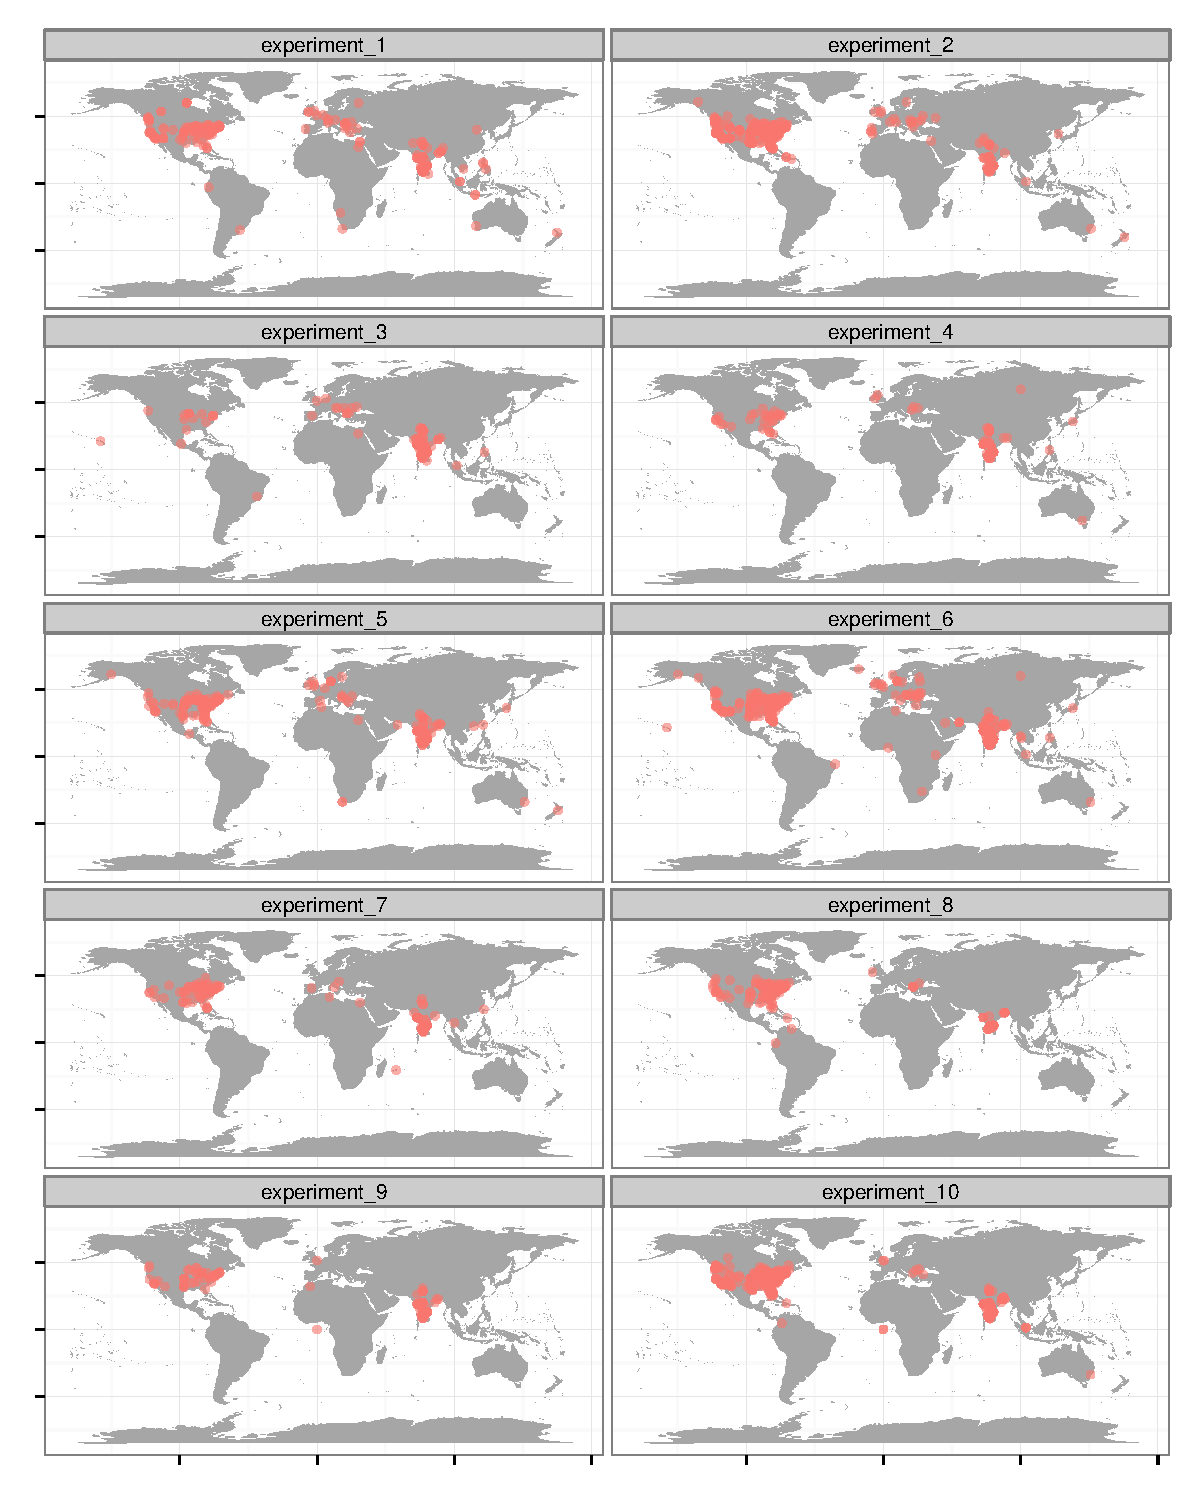
\includegraphics[width=6in]{turker_location_experiment.pdf} 
   \caption{World maps showing where the participants are coming from for all the 10 experiments.}
   \label{fig:turker_location_experiment}
\end{figure}





\begin{figure}[htbp] 
   \centering
   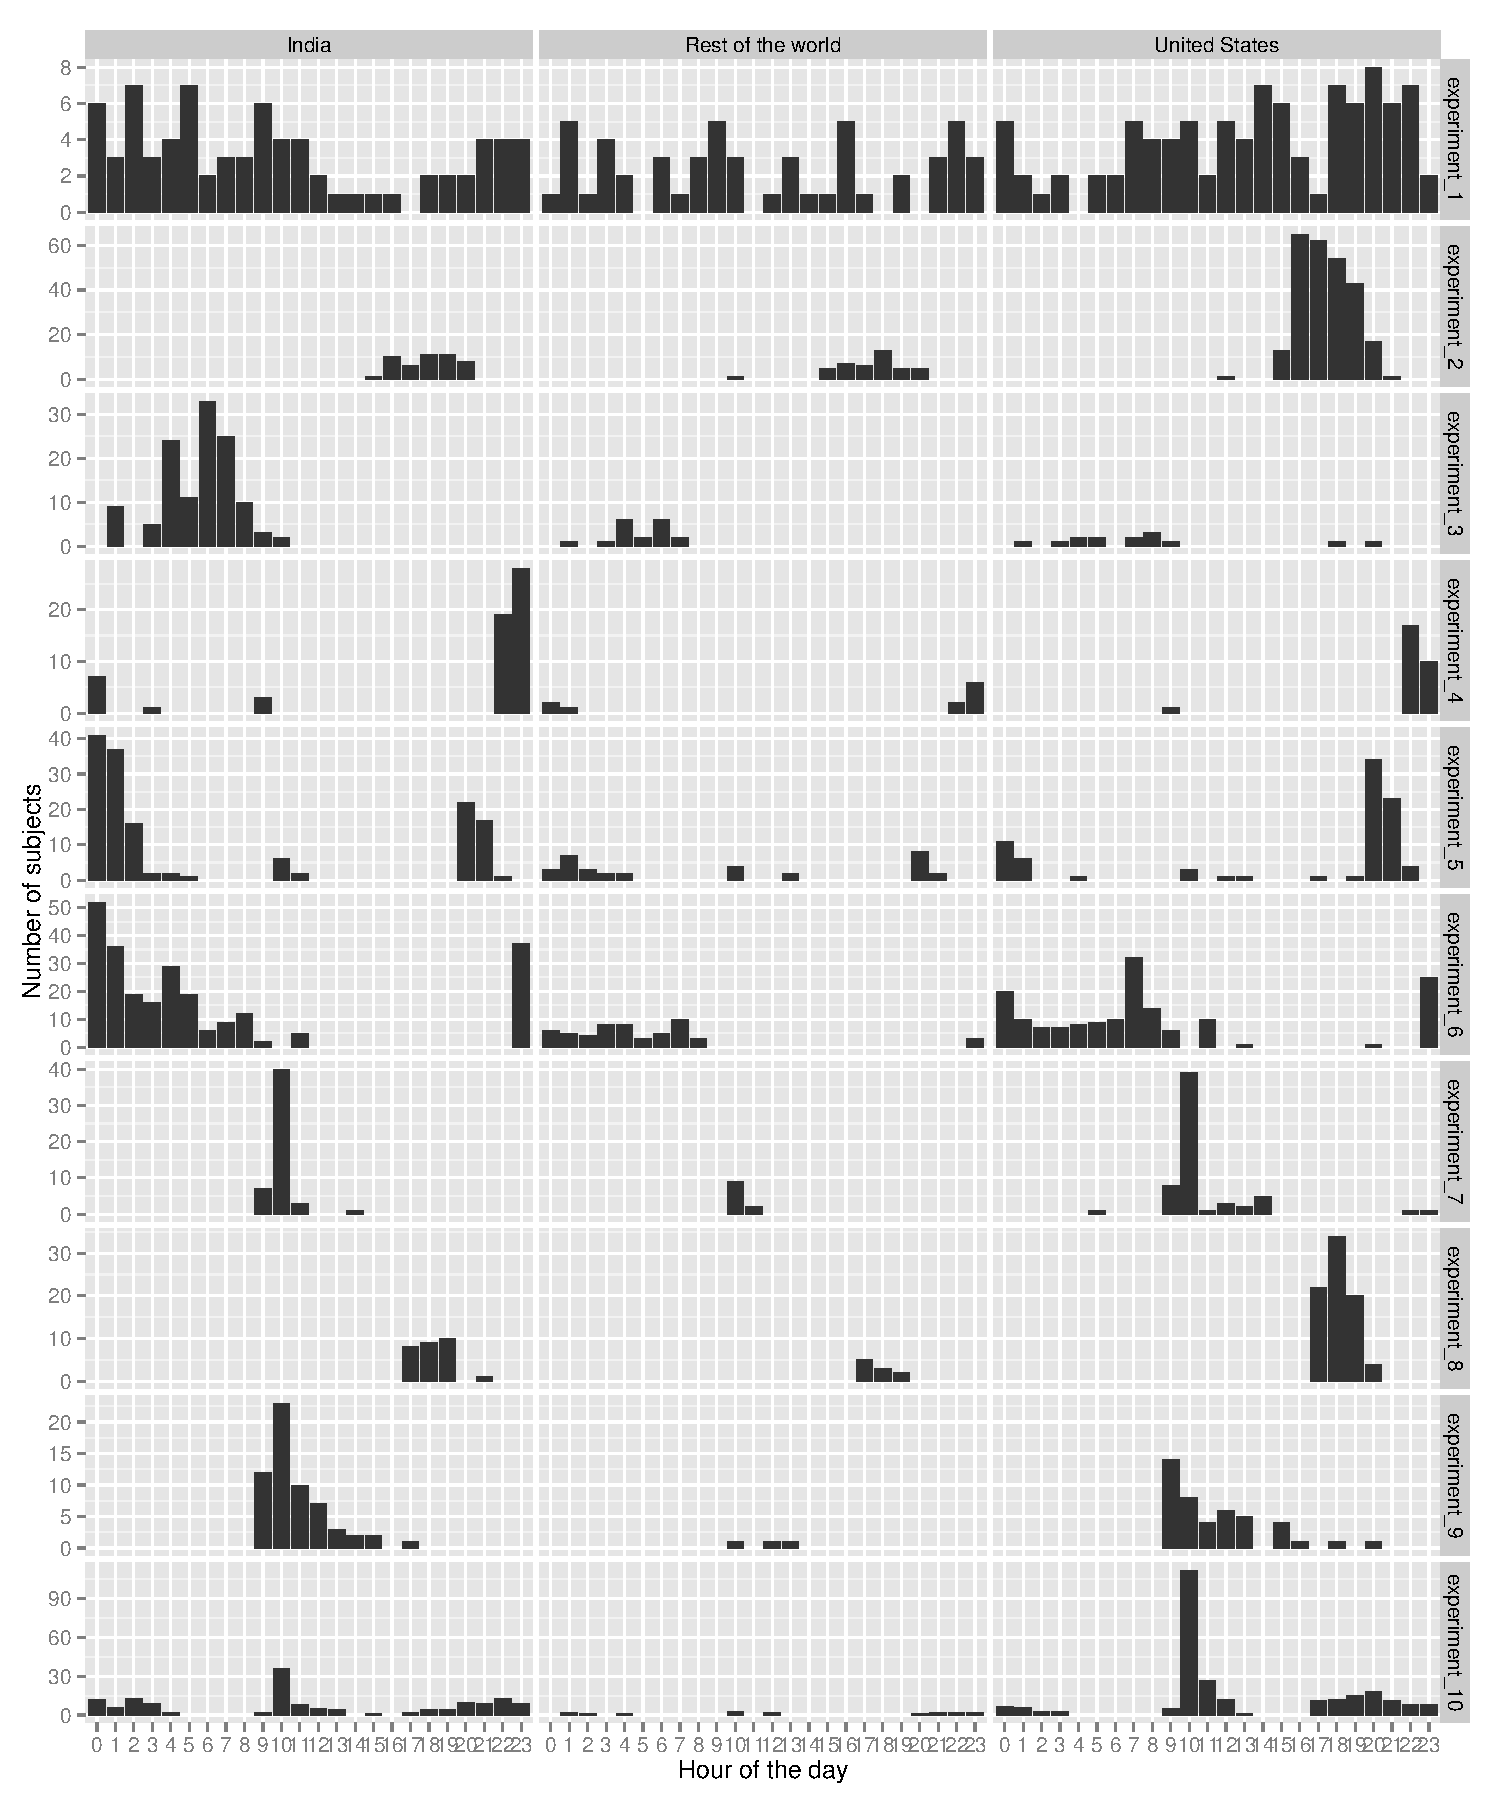
\includegraphics[width=6.5in]{participation_time.pdf} 
   \caption{Time of the day when the participants work (central time). Experiment 1 shows MTurk workers participated the experiments around the clock. Other experiments did not take a whole day to finish. For experiment 3 most of the participants are from India because of timing. No matter when the experiment is started, subjects from India shows participations. For United States, subjects participated if the experiment is not in the mid night, except for experiment 6.}
   \label{fig:participation_time}
\end{figure}

\clearpage
\section{Electoral Building Lineups and Results}
Figures~\ref{fig:elect.1} through~\ref{fig:elect.5} show the five lineups shown to (different) Amazon Turk workers in an experiment. They all are created as described in the introduction of the paper. In order to not bias observers, no context information was given about how these plots were created or what data they were displaying. This also made it necessary to slightly more stylize the display. 

% latex table generated in R 3.0.1 by xtable 1.7-1 package
% Wed Jun  5 17:39:09 2013
\begin{table}[hbtp]
\centering
\begin{tabular}{rrrrrr}
  \hline
 lineup & \#1 & \#2 & \#3 & \#4 & \#5 \\ 
  \hline
  \# correct/ \#evaluation &  12/72 & 11/66 & 5/74 & 14/72 & 19/57 \\ 
$p$-value & 0.00023 & 0.00041 & 0.31 & 1.2e-05 &  1.9e-11 \\ 
data panel & $3\cdot4+1$ & $2^4+1$ & $4^2+2 $ & $12+\sqrt{25}$ & $2^3-7$ \\ 
   \hline
\end{tabular}
\end{table}

% latex table generated in R 3.0.1 by xtable 1.7-1 package
% Wed Jun  5 18:00:55 2013
\begin{table}[hbtp]
\centering
\caption{\label{tbl:response}Overview of all choices by observers for each of the lineups. The correct choice is bolded. In most lineups there are null plots that were picked more often by observers, but the actual result is among the plots being picked most often, indicating that there is some indication that the election result is not completely consistent with the polls.}
\begin{tabular}{rrrrrrrrrrrrrrrrrrrrr}
  \hline
& \multicolumn{10}{l}{panel chosen}\\
Lineup & 1 & 2 & 3 & 4 & 5 & 6 & 7 & 8 & 9 & 10 & 11 & 12 & 13 & 14 & 15 & 16 & 17 & 18 & 19 & 20 \\ 
  \hline
\#  1 & 2 & 2 & 0 & 10 & 2 & 2 & 6 &  23 & 1 & 1 & 0 & 1 & \bf 12 & 3 & 3 & 1 & 0 & 1 & 1 & 1 \\ 
\#  2 & 0 & 16 & 1 & 1 & 5 & 1 & 0 & 8 & 0 & 2 & 0 & 0 & 0 & 4 & 2 & 1 & \bf 11 & 1 & 0 & 13 \\ 
\#  3 & 7 & 26 & 0 & 2 & 0 & 5 & 3 & 0 & 2 & 1 & 0 & 4 & 0 & 0 & 2 & 0 & 9 & \bf 5 & 0 & 6 \\ 
\#  4 & 0 & 0 & 0 & 2 & 0 & 0 & 0 & 3 & 1 & 10 & 2 & 18 & 1 & 0 & 4 & 2 &\bf 14 & 0 & 13 & 0 \\ 
\# 5 &\bf 19 & 1 & 4 & 1 & 0 & 1 & 0 & 12 & 0 & 0 & 0 & 4 & 1 & 0 & 0 & 12 & 1 & 1 & 0 & 0 \\ 
   \hline
\end{tabular}
\end{table}

\begin{figure}[htbp] 
   \centering
   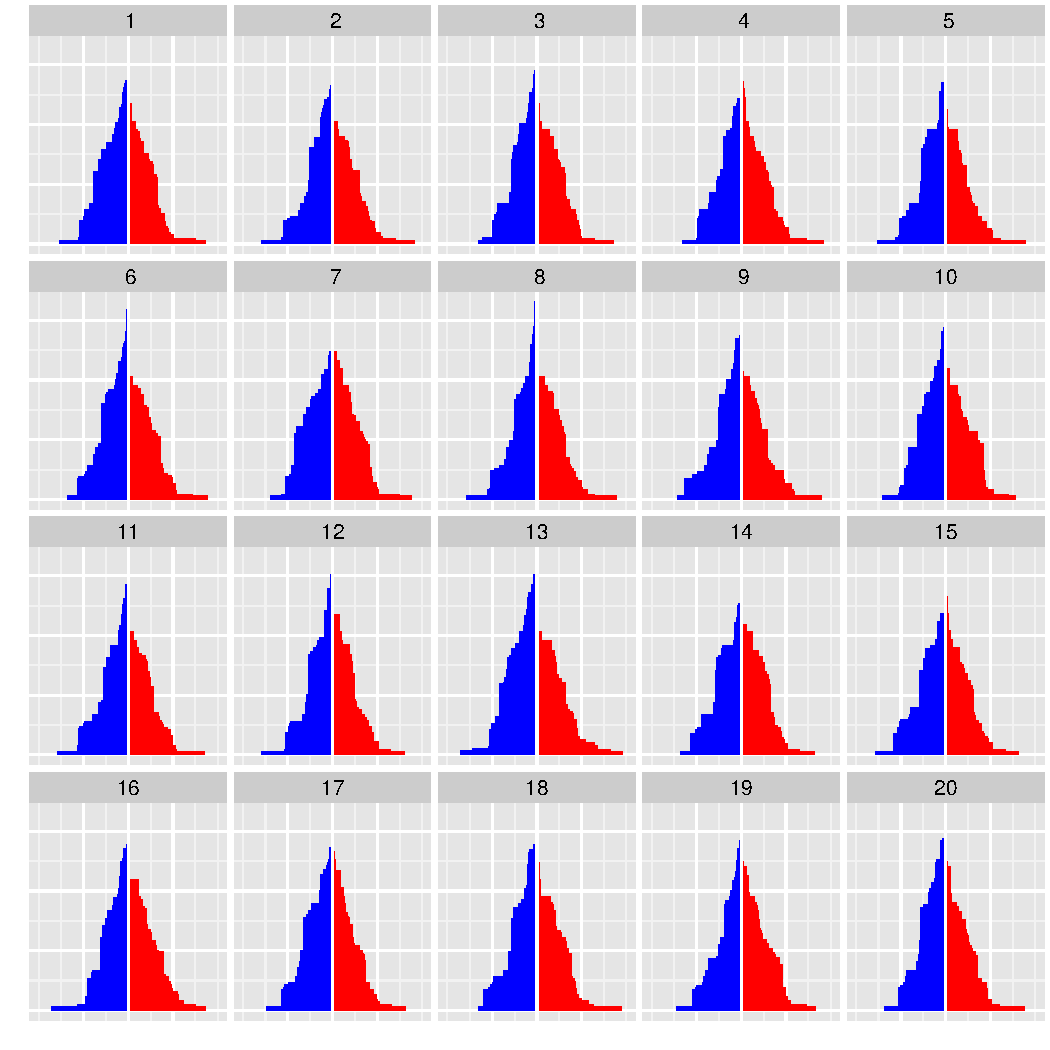
\includegraphics[width=0.8\linewidth]{electoral-5-13.pdf} 
   \caption{Lineup \#1 - electoral building. Which building looks the most different from the other buildings? }
   \label{fig:elect.1}
\end{figure}

\begin{figure}[htbp] 
   \centering
   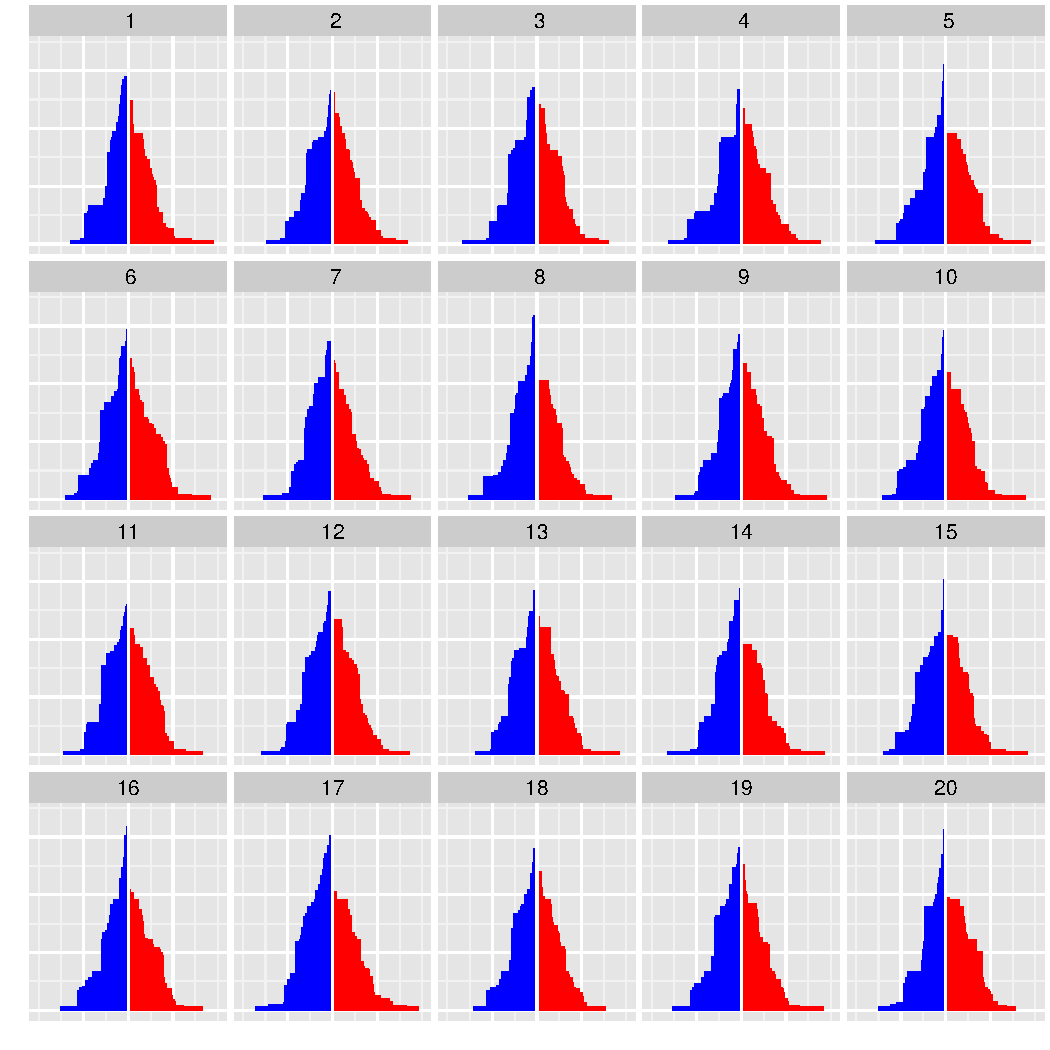
\includegraphics[width=0.8\linewidth]{electoral-2-17.pdf} 
   \caption{Lineup \#2 - electoral building. Which building looks the most different from the other buildings? }
   \label{fig:elect.2}
\end{figure}
\begin{figure}[htbp] 
   \centering
   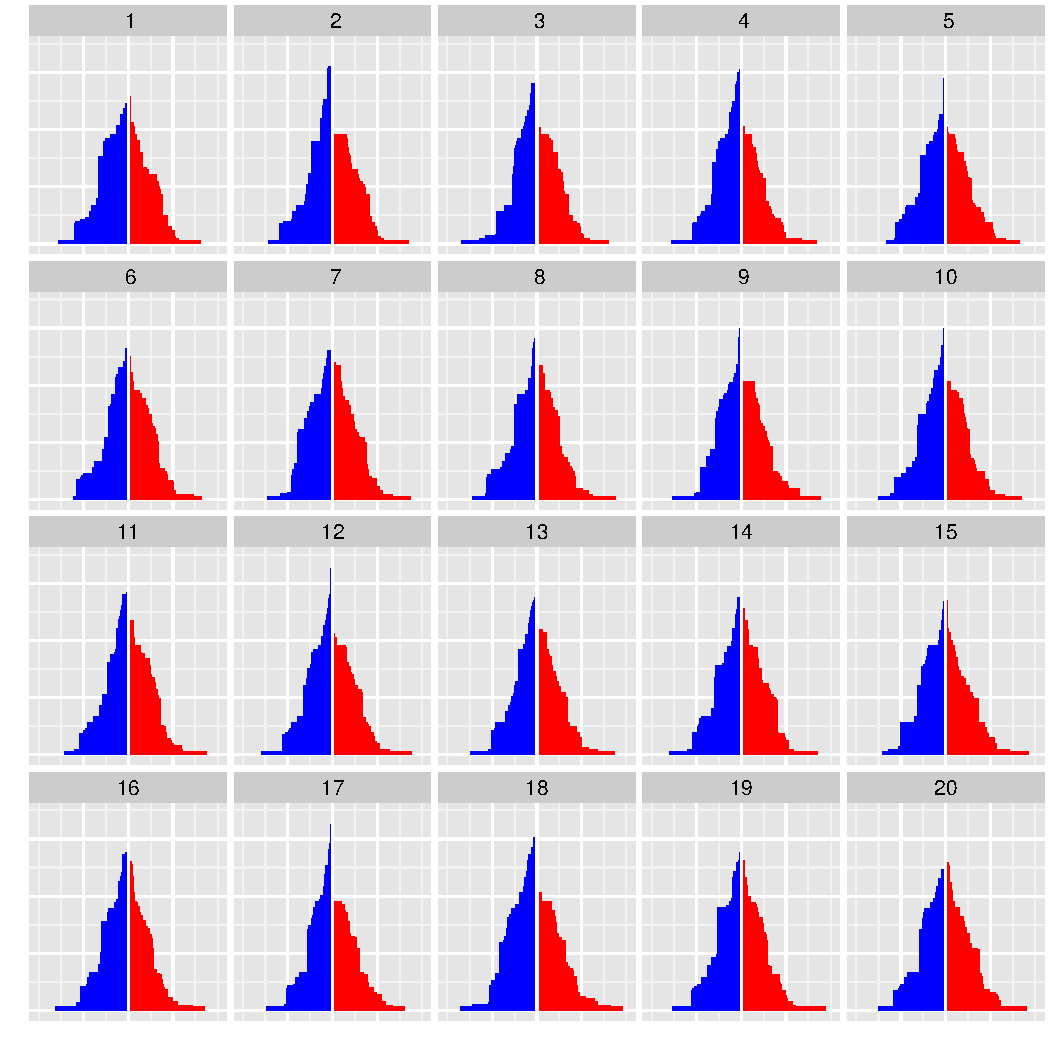
\includegraphics[width=0.8\linewidth]{electoral-3-18.pdf} 
   \caption{Lineup \#3 - electoral building. Which building looks the most different from the other buildings? }
   \label{fig:elect.3}
\end{figure}
\begin{figure}[htbp] 
   \centering
   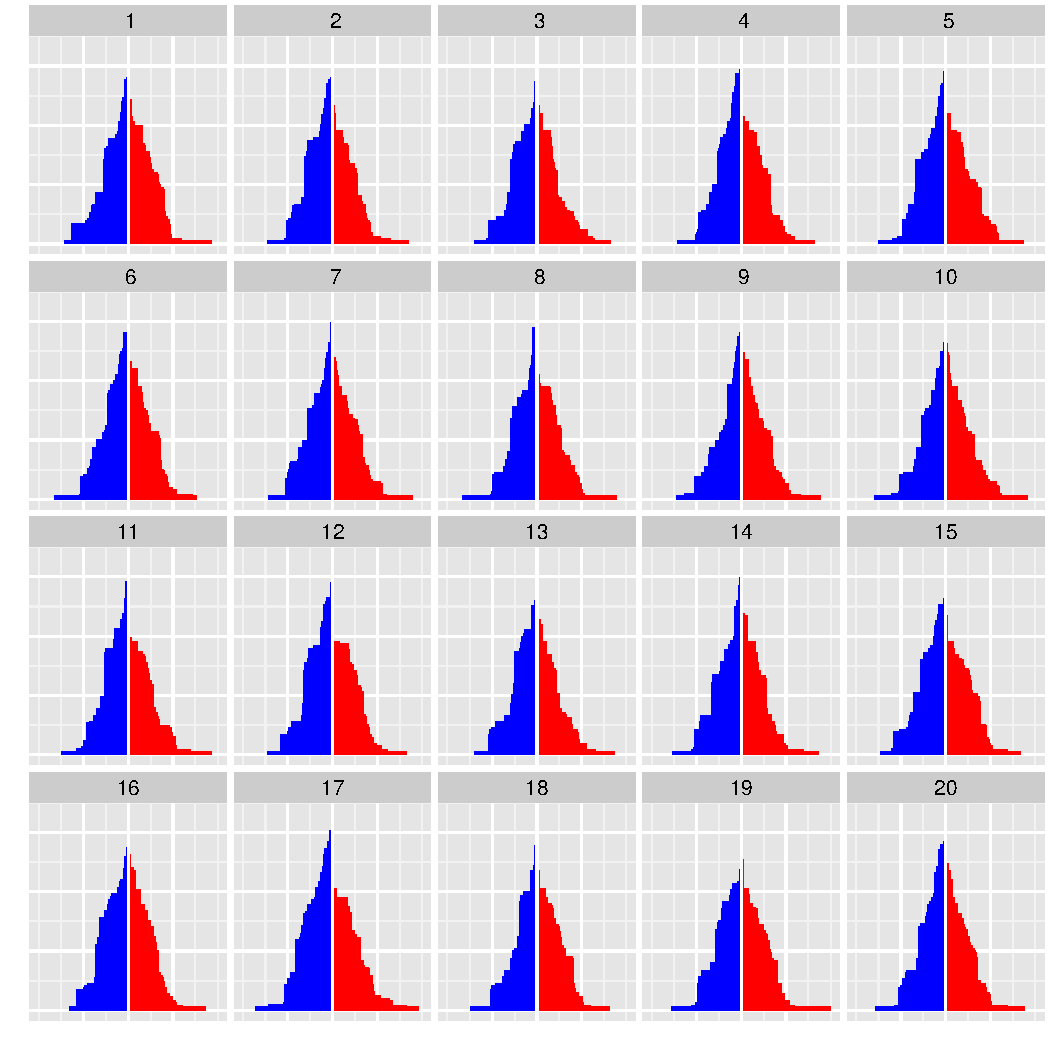
\includegraphics[width=0.8\linewidth]{electoral-4-17.pdf} 
   \caption{Lineup \#4 - electoral building. Which building looks the most different from the other buildings? }
   \label{fig:elect.4}
\end{figure}
\begin{figure}[htbp] 
   \centering
   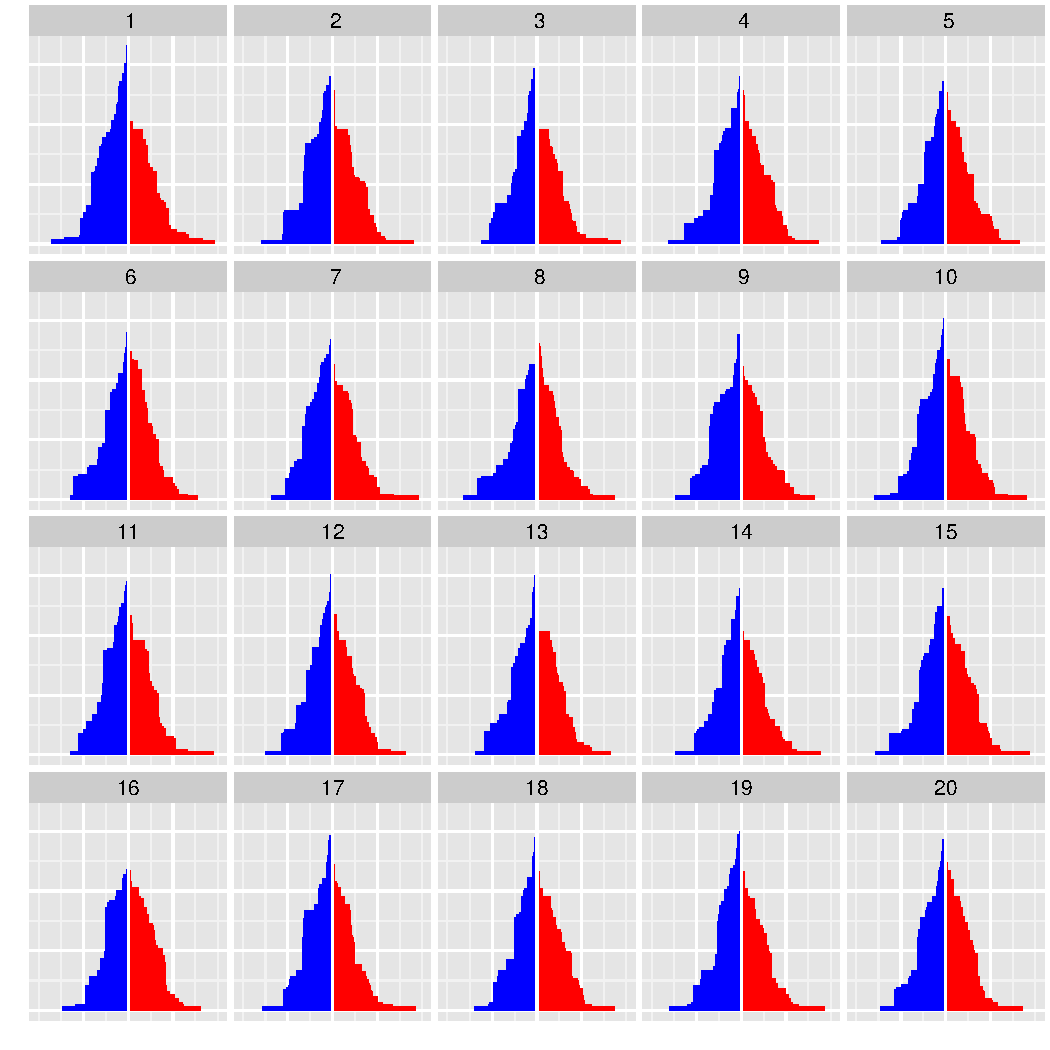
\includegraphics[width=0.8\linewidth]{electoral-1-1.pdf} 
   \caption{Lineup \#5 - electoral building. Which building looks the most different from the other buildings? }
   \label{fig:elect.5}
\end{figure}



\bibliographystyle{asa}
\bibliography{references}

\end{document}



